\chapter{Methods of Integration}
%Begin Section 6.1
\section{Integration by Parts}
In physics and engineering the
\textbf{Gamma function}\index{Gamma function}\footnote{Created by the Swiss
mathematician, physicist and astronomer Leonhard Euler (1707-1783). The use of
the Greek capital letter $\Gamma$ for this function is due to the French
mathematician Adrien-Marie Legendre (1752-1833).}
 $\Gamma\,(t)$, defined by
\[
\Gamma\,(t) ~=~ \int_0^{\infty} x^{t-1} \, e^{-x} ~\dx \quad\text{for all $t > 0$,}
\]
has found many uses. Evaluating $\Gamma\,(2)$ entails integrating the function
$f(x) = x\,e^{-x}$. No formula or substitution you have learned so far would be
of help. \emph{Differentiating} that function, on the other hand, is easy. By
the Product Rule for differentials,
\begin{align*}
d(x\,e^{-x}) ~&=~ x\,d(e^{-x}) ~+~ d(x)\,e^{-x}\\
&=~ -x\,e^{-x}\,\dx ~+~ e^{-x}\,\dx\\
d(x\,e^{-x}) ~&=~ -x\,e^{-x}\,\dx ~-~ d(e^{-x})\\
x\,e^{-x}\,\dx ~&=~ -d(x\,e^{-x}) ~-~ d(e^{-x}),\quad\text{so integrate both sides to get}\\[6pt]
\int x\,e^{-x}\,\dx ~&=~ -\int d(x\,e^{-x}) ~-~ \int d(e^{-x})
~=~ -x\,e^{-x} ~-~ e^{-x} ~+~ C
\end{align*}
since $\int d\!F \,=\, F \,+\, C$. Generalizing this process for functions $u$
and $v$,
\begin{align*}
d(uv) ~&=~ u\,\dv ~+~ v\,\du\\
u\,\dv ~&=~ d(uv) ~-~ v\,\du
\end{align*}
so that integrating both sides yields the \textbf{integration by parts}
formula:\index{integration!by parts}

\statethm{thm:intbyparts}{For differentiable functions $u$ and $v$:
\begin{equation}
\int u\,\dv ~=~ uv ~-~ \int v\,\du
\end{equation}}
Integration by parts is just the Product Rule for derivatives in integral form,
typically used when the integral $\int v\,\du$ would be simpler than the
original integral $\int u\,\dv$.

\begin{exmp}\label{exmp:intparts1}
\noindent Use integration by parts to evaluate
$~\displaystyle\int x\,e^{-x}\,\dx~$. Use the answer to evaluate
$\Gamma\,(2)$.\vspace{1mm}
\par\noindent\emph{Solution:} The original integral is always of the form
$\int u\,\dv$, so you must decide which parts of $x e^{-x}\,\dx$ will represent
$u$ and $\dv$. Typically you would choose $\dv$ to be a
differential that you could integrate easily (since you will need to integrate
$\dv$ to get $v$) and choose $u$ to be a function whose
derivative is simpler than $u$ (since that derivative will appear in $v\,\du$,
which you hope to be a simpler integral). In this case, pick $u = x$ and
$\dv = e^{-x}\,\dx$. Then $\du = \dx$ and
$v = \int \dv = \int e^{-x}\,\dx = -e^{-x}$ (you can omit the generic constant
$C$ for now---include it when you have evaluated $\int v\,\du$). Thus,
\begin{align*}
\int u\,\dv ~&=~ uv ~-~ \int v\,\du\\[6pt]
\int \underbracket[0.3pt]{x\vphantom{\tfrac{1}{2}}}_{u\vphantom{d}}\,\underbracket[0.3pt]{e^{-x}\,\dx\vphantom{\tfrac{1}{2}}}_{\dv} ~&=~
 \underbracket[0.3pt]{x\vphantom{\tfrac{1}{2}}}_{u\vphantom{d}}\,\underbracket[0.3pt]{(-e^{-x})\vphantom{\tfrac{1}{2}}}_{v\vphantom{d}} ~-~
 \int \underbracket[0.3pt]{-e^{-x}\vphantom{\tfrac{1}{2}}}_{v\vphantom{d}}\,\underbracket[0.3pt]{\dx\vphantom{\tfrac{1}{2}}}_{\du}\\[6pt]
\int x\,e^{-x}\,\dx ~&=~ -x\,e^{-x} ~-~ e^{-x} ~+~ C
\end{align*}
which agrees with the example at the beginning of this section. Note that
$\int v\,\du = \int -e^{-x}\,\dx$, which indeed is simpler than the original
integral. The Gamma function value $\Gamma\,(2)$ can now be evaluated:
\begin{align*}
\Gamma\,(2) ~&=~ \int_0^{\infty} x\,e^{-x}\,\dx\\
&=~ -x\,e^{-x} ~-~ e^{-x}~\Biggr|_{0}^{\infty}\\[4pt]
&=~ \lim_{x \to \infty}~(-x\,e^{-x} ~-~ e^{-x}) ~-~ (-0\,e^{0} ~-~ e^{0})\\[4pt]
&=~ -\left(\lim_{x \to \infty}~\frac{x}{e^x}\right) ~-~ \left(\lim_{x \to \infty}~e^{-x}\right) ~-~ (0 - 1)\\[4pt]
&=~ 0 ~-~ 0 ~+~ 1 ~=~ 1
\end{align*}
\end{exmp}
\begin{exmp}\label{exmp:intparts2}
\noindent What would happen in Example \ref{exmp:intparts1} if you let
$u = e^{-x}$ and $\dv = x\,\dx$?\vspace{1mm}
\par\noindent\emph{Solution:} In this case $\du = -e^{-x}\,\dx$ and
$v = \int \dv = \int x\,\dx = \frac{1}{2}x^2$, so that
\begin{align*}
\int x\,e^{-x}\,\dx ~&=~ \int \underbracket[0.3pt]{e^{-x}\vphantom{\tfrac{1}{2}}}_{u\vphantom{d}}\,\underbracket[0.3pt]{x~\dx\vphantom{\tfrac{1}{2}}}_{\dv}\\[6pt]
&=~ \underbracket[0.3pt]{e^{-x}\vphantom{\frac{1}{2}}}_{u\vphantom{d}}\,\underbracket[0.3pt]{\frac{1}{2}x^2}_{v\vphantom{d}} ~-~
 \int \underbracket[0.3pt]{\frac{1}{2}x^2}_{v\vphantom{d}}\,\underbracket[0.3pt]{(-e^{-x})\,\dx\vphantom{\frac{1}{2}}}_{\du}\\[6pt]
&=~ \frac{1}{2}x^2\,e^{-x} ~+~ \frac{1}{2}\,\int x^2\,e^{-x}\,\dx
\end{align*}
which leads you in the wrong direction: a more difficult integral than the
original.
\end{exmp}\vspace{-2mm}
\divider
\newpage
Example \ref{exmp:intparts2} showed the importance of an appropriate choice for
$u$ and $\dv$. There are some rough guidelines for that choice---as in
Example \ref{exmp:intparts1}---but no rules that are guaranteed to always work.
It might not be clear when you should even attempt integration by parts.

\begin{exmp}\label{exmp:intparts3}
\noindent Evaluate $~\displaystyle\int \ln x~\dx~$.\vspace{1mm}
\par\noindent\emph{Solution:} Integration by parts ostensibly requires two
functions in the integral, whereas here $\ln x$ appears to be the only one.
However, the choice for $\dv$ is a \emph{differential}, and one exists here:
$\dx$. Choosing $\dv = \dx$ obliges you to let $u = \ln\,x$. Then
$\du = \frac{1}{x}\;\dx$ and $v = \int \dv = \int \dx = x$. Now integrate by
parts:
\begin{align*}
\int u\,\dv ~&=~ uv ~-~ \int v\,\du\\[6pt]
\int \ln\,x~\dx ~&=~ (\ln\,x)\,(x) ~-~ \int x \cdot \frac{1}{x}~\dx\\[6pt]
&=~ x\,\ln\,x ~-~ \int 1~\dx\\[6pt]
&=~ x\,\ln\,x ~-~ x ~+~ C
\end{align*}
Note that choosing $\dv = \ln\,x\;\dx$ would be pointless, as integrating
$\dv$ to get $v$ is the original problem!
\end{exmp}
\begin{exmp}\label{exmp:intparts4}
\noindent Evaluate $~\displaystyle\int x^3\,e^{x^2}\,\dx~$.\vspace{1mm}
\par\noindent\emph{Solution:} One frequently useful guideline for integration
by parts is to eliminate the most complicated function in the integral by
integrating it---as $\dv$---into something simpler (which becomes $v$). In
this integral, $e^{x^2}$ is somewhat complicated but has no
closed form antiderivative. However, $x\,e^{x^2}$ appears in the
integral and can be integrated easily (using a substitution as in Section 5.4).
So choose $\dv = x\,e^{x^2}\,\dx$, which means $u = x^2$. Then
$\du = 2x\,\dx$ and $v = \int \dv = \int x\,e^{x^2}\,\dx = \frac{1}{2}e^{x^2}$.
Now integrate by parts:
\begin{align*}
\int u\,\dv ~&=~ uv ~-~ \int v\,\du\\[6pt]
\int x^3\,e^{x^2}\,\dx ~&=~ x^2\,\cdot\,\frac{1}{2}\,e^{x^2} ~-~
\int \frac{1}{2}\,e^{x^2} \cdot 2x~\dx\\[6pt]
&=~ \frac{x^2}{2}\,e^{x^2} ~-~ \int x\,e^{x^2}\,\dx\\[6pt]
&=~ \frac{x^2}{2}\,e^{x^2} ~-~ \frac{1}{2}\,e^{x^2} ~+~ C\\[6pt]
&=~ \frac{(x^2 - 1)}{2}\,e^{x^2} ~+~ C
\end{align*}
\end{exmp}
\divider
\vspace{2mm}
Sometimes multiple rounds of integration by parts are needed, as in the
following example.
\newpage
\begin{exmp}\label{exmp:intparts5}
\noindent Evaluate $~\displaystyle\int x^2\,e^{-x}\,\dx~$.\vspace{1mm}
\par\noindent\emph{Solution:} This integral appears similar to the one in
Example \ref{exmp:intparts1}, so choose $\dv = e^{-x}\,\dx$ and $u = x^2$. Then
$\du = 2x\,\dx$ and $v = \int e^{-x}\,\dv = -e^{-x}$. Now integrate by parts:
\begin{align*}
\int u\,\dv ~&=~ uv ~-~ \int v\,\du\\[6pt]
\int x^2\,e^{-x}\,\dx ~&=~ x^2\,\cdot\,(-e^{-x}) ~-~
 \int -e^{-x} \cdot 2x~\dx\\[6pt]
&=~ -x^2\,e^{-x} ~+~ 2\,\int x\,e^{-x}\,\dx\quad\text{(integrate by parts \emph{again})}\\[4pt]
\int x^2\,e^{-x}\,\dx ~&=~ -x^2\,e^{-x} ~+~
 2\,(-x\,e^{-x} ~-~ e^{-x}) ~+~ C\quad\text{(by Example \ref{exmp:intparts1})}\\
&=~ -x^2\,e^{-x} ~-~ 2x\,e^{-x} ~-~ 2\,e^{-x} ~+~ C
\end{align*}
\end{exmp}\vspace{-2mm}
\divider
\vspace{2mm}

In the above example, notice that the $u=2x$ in the second integral came from
the derivative of the $u=x^2$ in the first integral. Likewise, the
$\dv =-e^{-x}\,\dx$ in the second integral came from integrating the
$\dv=e^{-x}\,\dx$ in the first integral. In general, if $n$ rounds of
integration by parts were needed, with $u_i$ and $v_i$ representing the $u$ and
$v$, respectively, for round $i =1$, $2$, $\ldots$, $n$, then the repeated
integration by parts would look like this:
\begin{align*}
\int u_1\,\dv_1 ~&=~ u_1v_1 ~-~ \int v_1\,\du_1\\[6pt]
&=~ u_1v_1 ~-~ \int u_2\,\dv_2\\[6pt]
&=~ u_1v_1 ~-~ \left(u_2v_2 ~-~ \int v_2\,\du_2\right) ~=~
    u_1v_1 ~-~ u_2v_2 ~+~ \int u_3\,\dv_3\\[6pt]
&=~ u_1v_1 ~-~ u_2v_2 ~+~ \left(u_3v_3 ~-~ \int u_4\,\dv_4\right)\\[6pt]
&=~ u_1v_1 ~-~ u_2v_2 ~+~ u_3v_3 ~-~ \left(u_4v_4 ~-~ \int u_5\,\dv_5\right)\\[6pt]
&=~ \cdots\\[6pt]
&=~ u_1v_1 ~-~ u_2v_2 ~+~ u_3v_3 ~-~ u_4v_4 ~+~ u_5v_5 ~-~ \cdots ~ \int u_n\,\dv_n
\end{align*}
The last integral $\int u_n\,\dv_n$ is one you could presumably integrate
easily.
\newpage
The above procedure is called the
\textbf{tabular method}\index{integration!tabular method}\index{tabular
integration} for integration by parts, since it can be shown in a table (the
arrows indicate multiplication):

\begin{center}
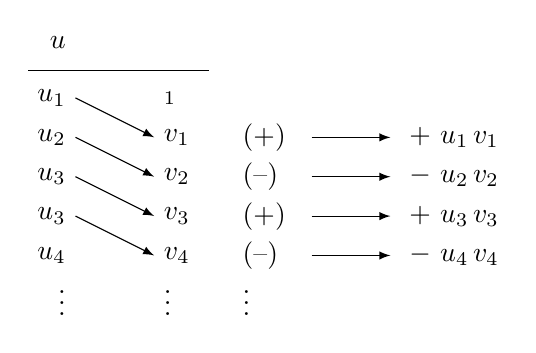
\begin{tikzpicture}[>=latex]
 \node[left] at (0,0.2) {$u$};
 \node[right] at (1,0.2) {$\dv$};
 \draw (-0.6,-0.15) -- (1.7,-0.15);

 \node[left] at (0,-0.5) {$u_1$};
 \node[right] at (1,-0.5) {$\dv_1$};
 \node[left] at (0,-1) {$u_2$};
 \node[right] at (1,-1) {$v_1$};
 \draw[->] (0,-0.5) -- (1,-1);
 \node[right] at (2,-1) {(+)};
 \draw[->] (3,-1) -- (4,-1) node[right] {$~+~u_1\,v_1$};

 \node[left] at (0,-1.5) {$u_3$};
 \node[right] at (1,-1.5) {$v_2$};
 \draw[->] (0,-1) -- (1,-1.5);
 \node[right] at (2,-1.5) {(--)};
 \draw[->] (3,-1.5) -- (4,-1.5) node[right] {$~-~u_2\,v_2$};

 \node[left] at (0,-2) {$u_3$};
 \node[right] at (1,-2) {$v_3$};
 \draw[->] (0,-1.5) -- (1,-2);
 \node[right] at (2,-2) {(+)};
 \draw[->] (3,-2) -- (4,-2) node[right] {$~+~u_3\,v_3$};


 \node[left] at (0,-2.5) {$u_4$};
 \node[right] at (1,-2.5) {$v_4$};
 \draw[->] (0,-2) -- (1,-2.5);
 \node[right] at (2,-2.5) {(--)};
 \draw[->] (3,-2.5) -- (4,-2.5) node[right] {$~-~u_4\,v_4$};

 \node[left] at (0,-3) {$\vdots$};
 \node[right] at (1,-3) {$\vdots$};
 \node[right] at (2,-3) {$\vdots$};
\end{tikzpicture}
\end{center}

The idea is to differentiate down the $u$ column and integrate down the $\dv$
column. If the $u$ in the original integral is a polynomial of degree $n$, then
you know from Section 1.6 that its $(n+1)$-st derivative will be 0, at which
point the tabular method terminates. The integral is then the sum of the
indicated products with alternating signs.

For example, the tabular method on the integral from Example
\ref{exmp:intparts5} looks like this:

\begin{center}
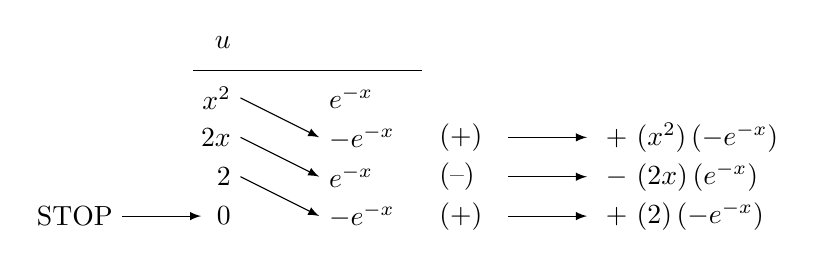
\begin{tikzpicture}[>=latex]
 \node[left] at (0,0.2) {$u$};
 \node[right] at (1,0.2) {$\dv$};
 \draw (-0.6,-0.15) -- (2.3,-0.15);

 \node[left] at (0,-0.5) {$x^2$};
 \node[right] at (1,-0.5) {$e^{-x}\,\dx$};
 \node[left] at (0,-1) {$2x$};
 \node[right] at (1,-1) {$-e^{-x}$};
 \draw[->] (0,-0.5) -- (1,-1);
 \node[right] at (2.4,-1) {(+)};
 \draw[->] (3.4,-1) -- (4.4,-1) node[right] {$~+~(x^2)\,(-e^{-x})$};

 \node[left] at (0,-1.5) {$2$};
 \node[right] at (1,-1.5) {$e^{-x}$};
 \draw[->] (0,-1) -- (1,-1.5);
 \node[right] at (2.4,-1.5) {(--)};
 \draw[->] (3.4,-1.5) -- (4.4,-1.5) node[right] {$~-~(2x)\,(e^{-x})$};

 \node[left] at (0,-2) {$0$};
 \node[right] at (1,-2) {$-e^{-x}$};
 \draw[->] (0,-1.5) -- (1,-2);
 \node[right] at (2.4,-2) {(+)};
 \draw[->] (3.4,-2) -- (4.4,-2) node[right] {$~+~(2)\,(-e^{-x})$};
 \draw[->] (-1.5,-2) node[left] {STOP~} -- (-0.5,-2);
\end{tikzpicture}
\end{center}
The integral is the sum of the products, and agrees with the result in Example
\ref{exmp:intparts5}:
\[
\int x^2\,e^{-x}\,\dx ~=~ +~(x^2)\,(-e^{-x}) ~-~(2x)\,(e^{-x}) ~+~(2)\,(-e^{-x}) ~+~ C
~=~ -x^2\,e^{-x} ~-~ 2x\,e^{-x} ~-~ 2\,e^{-x} ~+~ C
\]

\begin{exmp}\label{exmp:intparts6}
\noindent Evaluate $~\displaystyle\int x^3\,e^{-x}\,\dx~$.\vspace{1mm}
\par\noindent\emph{Solution:} Use the tabular method with $u = x^3$ and
$\dv = e^{-x}\,\dx$:
\begin{center}
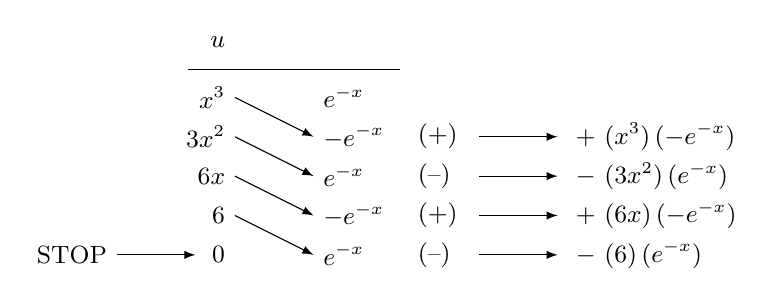
\begin{tikzpicture}[>=latex,every node/.style={font=\small}]
 \node[left] at (0,0.2) {$u$};
 \node[right] at (1,0.2) {$\dv$};
 \draw (-0.6,-0.15) -- (2.1,-0.15);

 \node[left] at (0,-0.5) {$x^3$};
 \node[right] at (1,-0.5) {$e^{-x}\,\dx$};
 \node[left] at (0,-1) {$3x^2$};
 \node[right] at (1,-1) {$-e^{-x}$};
 \draw[->] (0,-0.5) -- (1,-1);
 \node[right] at (2.2,-1) {(+)};
 \draw[->] (3.1,-1) -- (4.1,-1) node[right] {$~+~(x^3)\,(-e^{-x})$};

 \node[left] at (0,-1.5) {$6x$};
 \node[right] at (1,-1.5) {$e^{-x}$};
 \draw[->] (0,-1) -- (1,-1.5);
 \node[right] at (2.2,-1.5) {(--)};
 \draw[->] (3.1,-1.5) -- (4.1,-1.5) node[right] {$~-~(3x^2)\,(e^{-x})$};

 \node[left] at (0,-2) {$6$};
 \node[right] at (1,-2) {$-e^{-x}$};
 \draw[->] (0,-1.5) -- (1,-2);
 \node[right] at (2.2,-2) {(+)};
 \draw[->] (3.1,-2) -- (4.1,-2) node[right] {$~+~(6x)\,(-e^{-x})$};

 \node[left] at (0,-2.5) {$0$};
 \node[right] at (1,-2.5) {$e^{-x}$};
 \draw[->] (0,-2) -- (1,-2.5);
 \node[right] at (2.2,-2.5) {(--)};
 \draw[->] (3.1,-2.5) -- (4.1,-2.5) node[right] {$~-~(6)\,(e^{-x})$};
 \draw[->] (-1.5,-2.5) node[left] {STOP~} -- (-0.5,-2.5);
\end{tikzpicture}
\end{center}
\[
\int x^3\,e^{-x}\,\dx ~=~ -x^3\,e^{-x} ~-~ 3x^2\,e^{-x} ~-~ 6x\,e^{-x} ~-~ 6\,e^{-x} ~+~ C
\]
\end{exmp}\vspace{-2mm}
\divider
\newpage
Integration by parts can sometimes result in the original integral reappearing,
allowing it to be combined with the original integral.
\begin{exmp}\label{exmp:intparts7}
\noindent Evaluate $~\displaystyle\int \sec^3 x~\dx~$.\vspace{1mm}
\par\noindent\emph{Solution:} Let $u=\sec\,x$ and $\dv=\sec^2 x\;\dx$, so that
$\du = \sec\,x\;\tan\,x\;\dx$ and
$v = \int \dv = \int \sec^2 x\,\dx = \tan\,x$. Then
\begin{align*}
\int u\,\dv ~&=~ uv ~-~ \int v\,\du\\[6pt]
\int \sec^3 x~\dx ~&=~ \sec\,x\;\tan\,x ~-~ \int \sec\,x\;\tan^2 x~\dx\\[6pt]
\int \sec^3 x~\dx ~&=~ \sec\,x\;\tan\,x ~-~ \int \sec\,x\;(\sec^2 x \,-\, 1)~\dx\\[6pt]
\int \sec^3 x~\dx ~&=~ \sec\,x\;\tan\,x ~+~ \int \sec\,x~\dx ~-~ \int \sec^3 x~\dx\\[6pt]
2\,\int \sec^3 x~\dx ~&=~ \sec\,x\;\tan\,x ~+~
 \ln\;\abs{\,\sec\,x \;+\; \tan\,x\,} ~+~ C\\[6pt]
\int \sec^3 x~\dx ~&=~ \frac{1}{2}\,\left(\sec\,x\;\tan\,x ~+~
 \ln\;\abs{\,\sec\,x \;+\; \tan\,x\,}\right) ~+~ C
\end{align*}
\end{exmp}
\begin{exmp}\label{exmp:intparts8}
\noindent Evaluate $~\displaystyle\int e^x\,\sin\,x~\dx~$.\vspace{1mm}
\par\noindent\emph{Solution:} Let $u=e^x$ and $\dv=\sin\,x\,\dx$, so
that $\du = e^x\,\dx$ and $v = \int \dv = \int \sin\,x\,\dx = -\cos\,x$. Then
\begin{align*}
\int u\,\dv ~&=~ uv ~-~ \int v\,\du\\[6pt]
\int e^x\,\sin\,x~\dx ~&=~ -e^x\,\cos\,x ~+~ \int e^x\,\cos\,x~\dx
\end{align*}
and so integration by parts is needed again, for the integral on the right: let
$u=e^x$ and $\dv=\cos\,x\,\dx$, so that $\du = e^x\,\dx$ and
$v = \int \dv = \int \cos\,x\,\dx = \sin\,x$. Then
\begin{align*}
\int e^x\,\sin\,x~\dx ~&=~ -e^x\,\cos\,x ~+~ \left(uv ~-~ \int v\,\du\right)\\[6pt]
\int e^x\,\sin\,x~\dx ~&=~ -e^x\,\cos\,x ~+~ \left(e^x\,\sin\,x ~-~ \int e^x\,\sin\,x~\dx\right)\\[6pt]
2\,\int e^x\,\sin\,x~\dx ~&=~ -e^x\,\cos\,x ~+~ e^x\,\sin\,x\\[6pt]
\int e^x\,\sin\,x~\dx ~&=~ \frac{e^x}{2}\,(\sin\,x ~-~ \cos\,x) ~+~ C
\end{align*}
\end{exmp}
\divider
\newpage
In Example \ref{exmp:intparts1} integration by parts was used in evaluating an
improper integral. In general, in definite or improper integrals where $a$ and
$b$ are real numbers or $\pm\,\infty$,
\[
\int_a^b u\,\dv ~=~ uv~\Biggr|_a^b ~-~ \int_a^b v\,\du ~.
\]
\begin{exmp}\label{exmp:intparts9}
\noindent Evaluate $~\displaystyle\int_0^1 x^3\,\sqrt{1-x^2}~\dx~$.\vspace{1mm}
\par\noindent\emph{Solution:} Since
$x^3\,\sqrt{1-x^2} =x^2\,\cdot\,x\,\sqrt{1-x^2}$, and $x\,\sqrt{1-x^2}$
is easy to integrate (via a substitution), let  $u=x^2$ and
$\dv=x\,\sqrt{1-x^2}\,\dx$. Then $\du = 2x\,\dx$ and
$v = \int \dv = \int x\,\sqrt{1-x^2}\,\dx = -\frac{1}{3}(1-x^2)^{3/2}$, and so:
\begin{align*}
\int_a^b u\,\dv ~&=~ uv~\Biggr|_a^b ~-~ \int_a^b v\,\du\\[6pt]
\int_0^1 x^3\,\sqrt{1-x^2}~\dx ~&=~ -\frac{x^2}{3}(1-x^2)^{3/2}~\Biggr|_0^1 ~+~
 \int_0^1 \frac{2x}{3}(1-x^2)^{3/2}~\dx\\[6pt]
&=~ (0 - 0) ~+~ \left(\frac{-2}{15}(1-x^2)^{5/2}~\Biggr|_0^1\right) ~=~ 0 ~+~
 \frac{2}{15} ~=~ \frac{2}{15}
\end{align*}
\end{exmp}
\divider
\vspace{3mm}
\startexercises\label{sec6dot1}
{\small
\probs{A}
\par\noindent For Exercises 1-25, evaluate the given integral.
\begin{enumerate}[\bfseries 1.]
\begin{multicols}{5}
 \item $\displaystyle\int x\,\ln\,x~\dx$
 \item $\displaystyle\int x^2\,e^{x}\,\dx$
 \item $\displaystyle\int x\,\cos\,x~\dx$
 \item $\displaystyle\int x\,3^x\,\dx$
 \item $\displaystyle\int x^2\,a^x\,\dx~~(a>0)$
\end{multicols}
\begin{multicols}{5}
 \item $\displaystyle\int \ln\,4x~\dx$
 \item $\displaystyle\int \ln\,x^2~\dx$
 \item $\displaystyle\int x^2\,\sin\,x~\dx$
 \item $\displaystyle\int x\,\cos^2\,x~\dx$
 \item $\displaystyle\int \sin\,x\;\cos\,2x~\dx$
\end{multicols}
\begin{multicols}{5}
 \item $\displaystyle\int \sin^{-1} x~\dx$
 \item $\displaystyle\int \cos^{-1}\,2x~\dx$
 \item $\displaystyle\int \tan^{-1}\,3x~\dx$
 \item $\displaystyle\int x\,\sec^2 x~\dx$
 \item $\displaystyle\int \sin\,x\;\sin\,3x~\dx$
\end{multicols}
\begin{multicols}{5}
 \item $\displaystyle\int \frac{\ln\,x}{x^3}\,\dx\vphantom{\displaystyle\int_0^2 \frac{x^3\,\dx}{\sqrt{4 - x^2}}}$
 \item $\displaystyle\int x^3\,\ln^2 x~\dx\vphantom{\displaystyle\int_0^2 \frac{x^3\,\dx}{\sqrt{4 - x^2}}}$
 \item $\displaystyle\int x^5\,e^{x}\,\dx\vphantom{\displaystyle\int_0^2 \frac{x^3\,\dx}{\sqrt{4 - x^2}}}$
 \item $\displaystyle\int_0^2 \frac{x^3\,\dx}{\sqrt{4 - x^2}}$
 \item $\displaystyle\int_0^1 x^3\,\sqrt{1+x^2}\,\dx\vphantom{\displaystyle\int_0^2 \frac{x^3\,\dx}{\sqrt{4 - x^2}}}$
\end{multicols}
\begin{multicols}{5}
 \item $\displaystyle\int \sin\,(\ln\,x)~\dx$
 \item $\displaystyle\int \ln\,(1+x^2)\,\dx$
 \item $\displaystyle\int x\,\tan^{-1} x~\dx$
 \item $\displaystyle\int \cot^{-1}\,\sqrt{x}~\dx$
 \item $\displaystyle\int e^{\sqrt{x}}\,\dx$
\end{multicols}
 \item Evaluate the integral $\int e^x\,\sin\,x\,\dx$ from Example
 \ref{exmp:intparts8} by using two rounds of the tabular method and the formula
 $\int u_1\,\dv_1 = u_1v_1 - u_2v_2 + \int v_2\,\du_2$ from p.162.
\suspend{enumerate}
\probs{B}
\resume{enumerate}[{[\bfseries 1.]}]
 \item\label{exer:eaxtrigbx} Show that for all constants $a$ and $b \ne 0$ :
\begin{displaymath}
\int e^{ax}\,\cos\,bx~\dx ~=~ \frac{e^{ax}\,(a\,\cos\,bx \;+\; b\,\sin\,bx)}{a^2 + b^2} ~+~ C
\enskip\text{and}\enskip
\int e^{ax}\,\sin\,bx~\dx ~=~ \frac{e^{ax}\,(a\,\sin\,bx \;-\; b\,\cos\,bx)}{a^2 + b^2} ~+~ C
\end{displaymath}
\newpage
 \item\label{exer:gamma} For the Gamma function $\Gamma\,(t)$ show the following:
  \begin{enumerate}[\bfseries (a)]
   \item $\Gamma\,(t + 1) ~=~ t\,\Gamma\,(t)$ for all $t > 0$. \emph{(Hint:
    Use integration by parts.)}
   \item $\Gamma\,(n) ~=~ (n-1)\,!~$ for all positive integers $n$. \emph{(Hint:
    Use part (a) and induction.)}
  \end{enumerate}
 Note that by part (b) the Gamma function can be thought of as an extension of
 the factorial operation to all positive real numbers. In fact, the Gamma
 function was created for that purpose.
 \item Use Exercise \ref{exer:gamma} to prove for all integers $n \ge 1$:
\[
\int_0^{\infty} r^n\,e^{-r}\,\ln\,r~\dr ~=~
 (n-1)\,! ~+~ n\,\int_0^{\infty} r^{n-1}\,e^{-r}\,\ln\,r~\dr
\]
 \item By the \emph{Maxwell speed distribution} for gas molecules, the average
 speed $\avg{\nu}$ of molecules of mass $m$ in a gas at temperature $T$ is
\[
\avg{\nu} ~=~ 4\pi\,\left(\frac{m}{2\pi kT}\right)^{3/2}\;
              \int_0^{\infty} \nu^3\,e^{-m\nu^2/2kT}\,d\!\nu ~,
\]
where $k \approx 1.38056 \times 10^{-23}$ J/K is the Boltzmann constant. Show
that\index{Maxwell speed distribution}
\[
\avg{\nu} ~=~ \sqrt{\frac{8kT}{\pi m}} ~.
\]
 \item Some physics texts write integrals in a form like this energy integral
 from statistical mechanics,
\[
\int_0^{\infty} \ln\,\left(1 - \alpha e^{-x^2}\right)~d(x^3)
\]
which uses the differential of a \emph{function}---in this case
$d(x^3)$---instead of a variable (e.g. not just plain $\dx$). This often
signals that integration by parts is on the way, with the added benefit of
having the $v=\int \dv$ calculation done for you---in the above integral
$d(x^3)$ means that $v=x^3$, with $\dv=d(x^3)$ not really being needed for
anything else. With that understanding, show that for $0 < \alpha  < 1$,
\[
\int_0^{\infty} \ln\,\left(1 - \alpha e^{-x^2}\right)~d(x^3) ~=~
-2\alpha\,\int_0^{\infty} \frac{x^4\,e^{-x^2}\,\dx}{1 - \alpha e^{-x^2}} ~.
\]
 \item Find the flaw in the following ``proof'' that $0 = 1$:

\noindent\emph{Evaluating the integral}
$~\displaystyle\int \frac{\dx}{x}~$ \emph{using integration by parts with}
$u = \dfrac{1}{x}$ \emph{and} $\dv = \dx$, \emph{so that} 
$\du = -\dfrac{\dx}{x^2}$ \emph{and} $v = x$, 
\emph{shows that}
\begin{align*}
\int u\,\dv ~&=~ uv ~-~ \int v\,\du\\[6pt]
\int \frac{\dx}{x} ~&=~ \left(\frac{1}{x}\right) \,\cdot\,x ~-~ \int x \,\cdot\, \left(-\frac{\dx}{x^2}\right)\\[6pt]
\int \frac{\dx}{x} ~&=~ 1 ~+~ \int \frac{\dx}{x}\\[6pt]
0 ~&=~ 1 \quad\checkmark
\end{align*}
\end{enumerate}
}
\newpage
%Begin Section 6.2
\section{Trigonometric Integrals}
In engineering applications you sometimes encounter integrals of the form
\[
\int \cos\;(\alpha t + \phi_1)~\cos\;(\beta t + \phi_2)~\dt
\]
where $\alpha t + \phi_1$ and $\beta t + \phi_2$ are different angles (e.g. when
the voltage and current are out of phase in an AC circuit). In general,
integrals involving products of sines and cosines with ``mixed'' angles can be
simplified with the useful product-to-sum formulas:\footnote{See Section 3.4 in
\textsc{Corral, M.}, \emph{Trigonometry}, \url{http://mecmath.net/trig/}, 2009.}
\index{product-to-sum
formulas}\index{integral!trigonometric}\index{trigonometric integrals}
\begin{center}\statecomment{\vspace{-5mm}\begin{align}
 \sin\;A~\cos\;B ~&=~ \phantom{-}\tfrac{1}{2}\;(\sin\;(A+B) ~+~ \sin\;(A-B))\label{eqn:p2ssincos}\\
 \cos\;A~\sin\;B ~&=~ \phantom{-}\tfrac{1}{2}\;(\sin\;(A+B) ~-~ \sin\;(A-B))\label{eqn:p2scossin}\\
 \cos\;A~\cos\;B ~&=~ \phantom{-}\tfrac{1}{2}\;(\cos\;(A+B) ~+~ \cos\;(A-B))\label{eqn:p2scoscos}\\
 \sin\;A~\sin\;B ~&=~ -\tfrac{1}{2}\;(\cos\;(A+B) ~-~ \cos\;(A-B))\label{eqn:p2ssinsin}
\end{align}}\end{center}

\begin{exmp}\label{exmp:trigint1}
\noindent Evaluate $~\displaystyle\int 0.5\,\sin\,x\;\sin\,12x~\dx~$.\vspace{1mm}
\par\noindent\emph{Solution:} Using the product-to-sum formula
(\ref{eqn:p2ssinsin}) with $A=x$ and $B=12x$, 
\begin{align*}
\sin\;A~\sin\;B ~&=~ -\tfrac{1}{2}\;(\cos\;(A+B) ~-~ \cos\;(A-B))\\
\sin\,x~\sin\,12x ~&=~ -\tfrac{1}{2}\;(\cos\;(x+12x) ~-~ \cos\;(x-12x))\\
\sin\,x~\sin\,12x ~&=~ -\tfrac{1}{2}\;(\cos\,13x ~-~ \cos\,11x)
\end{align*}
since $\cos\,(-11x) = \cos\,11x$. Then
\begin{align*}
\int 0.5\,\sin\,x\;\sin\,12x~\dx ~&=~ -\frac{1}{4}\,\int (\cos\,13x ~-~ \cos\,11x)~\dx\\[6pt]
&=~ -\frac{1}{52}\,\sin\,13x ~+~ \frac{1}{44}\,\sin\,11x ~+~ C
\end{align*}
Notice how the product-to-sum formula turned an integral of products of sines
into integrals of individual cosines, which are easily integrated. The integrand
is an example of a \emph{modulated wave}\index{modulated wave}, commonly used in
electronic communications (e.g. radio broadcasting). The graph is shown below:
\begin{center}
\begin{tikzpicture}[>=latex,every node/.style={font=\small}]
 \draw [->,black!60,line width=1pt,anchor=base] (0,-0.7) -- (0,1) node[above] {$y$};
 \draw [->,black!60,line width=1pt,anchor=base] (0,0) -- (6.8,0) node[right] {$x$};
 \draw[black!60] (3.14,0) -- (3.14,-0.1);
 \draw[black!60] (6.28,0) -- (6.28,-0.1);
 \begin{scope}[dashed]
  \pgfplothandlerlineto
  \pgfplotfunction{\x}{0.00,0.01,...,6.29}{\pgfpointxy{\x}{-0.52*sin(\x r)}}
  \pgfplotfunction{\x}{0.00,0.01,...,6.29}{\pgfpointxy{\x}{0.52*sin(\x r)}}
  \pgfusepath{stroke}
 \end{scope}
 \begin{scope}[color=linecolor,line width=1.5pt]
  \pgfplothandlerlineto
  \pgfplotfunction{\x}{0.00,0.01,...,6.29}{\pgfpointxy{\x}{0.5*sin(\x r)*sin(12*\x r)}}
  \pgfusepath{stroke}
 \end{scope}
 \node[left] at (-0.1,0) {$0$};
 \node[left] at (-0.1,0.5) {$0.5$};
 \node[left] at (-0.1,-0.5) {$-0.5$};
 \draw[black!60] (0,0.5) -- (-0.1,0.5);
 \draw[black!60] (0,-0.5) -- (-0.1,-0.5);
 \node[above] at (3.14,0.6) {$y=0.5 \sin x\;\sin 12x$};
 \node[below] at (3.14,-0.1) {$\pi$};
 \node[below] at (6.28,-0.1) {$2\pi$};
\end{tikzpicture}
\end{center}
The curves $y=\pm 0.5 \sin\,x$ (shown in dashed lines) form an \emph{amplitude
envelope} for the modulated wave.
\end{exmp}\vspace{-2mm}
\divider
\newpage
On occasion you might need to integrate trigonometric functions raised to powers
higher than two. For the sine function raised to odd powers of the form $2n+1$
(for $n \ge 1$), the trick is to replace $\sin^2 x$ by $1 - \cos^2 x$, so that

\begin{align*}
\int \sin^{2n+1} x~\dx ~&=~ \int (\sin^2 x)^n \,\sin\,x~\dx\\[6pt]
&=~ \int (1 - \cos^2 x)^n \,\sin\,x~\dx\\[6pt]
&=~ \int p(u)~\du
\end{align*}
where $p(u)$ is a polynomial in the variable $u=\cos\,x$, and the remaining
single $\sin\,x$ is now part of $\du = -\sin\,x\;\dx$. You can then use the
Power Formula to integrate that polynomial.

\begin{exmp}\label{exmp:trigint2}
\noindent Evaluate $~\displaystyle\int \sin^3 x~\dx~$.\vspace{1mm}
\par\noindent\emph{Solution:} Let $u=\cos\,x$ so that $\du=-\sin\,x\;\dx$:
\begin{align*}
\int \sin^3 x~\dx ~&=~ \int (\sin^2 x) \;\sin\,x~\dx\\[6pt]
&=~ \int (1 - \cos^2 x) \;\sin\,x~\dx\\[6pt]
&=~ \int (1 - u^2)\;(-\du)\\[6pt]
&=~ \int (u^2 - 1)\;\du\\[6pt]
&=~ \frac{1}{3}\,u^3 ~-~ u ~+~ C\\[4pt]
&=~ \frac{1}{3}\,\cos^3 x ~-~ \cos\,x ~+~ C
\end{align*}
\end{exmp}
\divider
\vspace{2mm}
In general $\int \sin^{2n+1}\,x\;\dx$ will be a polynomial of degree $2n+1$ in
terms of $\cos\,x$. Similarly, use $\cos^2 x = 1 - \sin^2 x$ to integrate odd
powers of $\cos\,x$, with the substitution $u=\sin\,x$:
\begin{align*}
\int \cos^{2n+1} x~\dx ~&=~ \int (\cos^2 x)^n \,\cos\,x~\dx\\[6pt]
&=~ \int \underbracket[0.3pt]{(1 - \sin^2 x)^n\vphantom{\frac{1}{2}}}_{p(u)}
\;\underbracket[0.3pt]{\cos\,x~\dx\vphantom{\frac{1}{2}}}_{\du}
\end{align*}
\newpage
Integrals of the form $\int \sin^m\,x\;\cos^n\,x\;\dx$, where either $m$ or
$n$ is odd, can be evaluated using the above trick for the function having the
odd power.
\begin{exmp}\label{exmp:trigint3}
\noindent Evaluate $~\displaystyle\int \sin^2 x\;\cos^3 x~\dx~$.\vspace{1mm}
\par\noindent\emph{Solution:} Replace $\cos^2 x$ by $1 - \sin^2 x$, then let
$u=\sin\,x$ so that $\du=\cos\,x\;\dx$:
\begin{align*}
\int \sin^2 x\;\cos^3 x~~\dx ~&=~ \int \sin^2 x ~(\cos^2 x) \;\cos\,x~\dx\\[6pt]
&=~ \int \underbracket[0.3pt]{\sin^2 x ~(1 - \sin^2 x)\vphantom{\frac{1}{2}}}_{p(u)}
    \;\underbracket[0.3pt]{\cos\,x~\dx\vphantom{\frac{1}{2}}}_{\du}\\[3pt]
&=~ \int (u^2 - u^4)\;\du\\[6pt]
&=~ \frac{1}{3}\,u^3 ~-~ \frac{1}{5}\,u^5 ~+~ C\\[4pt]
&=~ \frac{1}{3}\,\sin^3 x ~-~ \frac{1}{5}\,\sin^5 x ~+~ C
\end{align*}
\end{exmp}
\divider
\vspace{2mm}
For even powers of $\sin\,x$ or $\cos\,x$. You would replace $\sin^2 x$ or
$\cos^2 x$ with either
\[
\sin^2 x ~=~ \frac{1 \;-\; \cos\,2x}{2} \quad\quad\text{or}\quad\quad
\cos^2 x ~=~ \frac{1 \;+\; \cos\,2x}{2} ~,
\]
respectively, as often as necessary, then proceed as before if odd powers occur.

\begin{exmp}\label{exmp:trigint4}
\noindent Evaluate $~\displaystyle\int \sin^4 x ~\dx~$.\vspace{1mm}
\par\noindent\emph{Solution:} Replace $\sin^2 x$ by $\frac{1 - \cos\,2x}{2}$:
\begin{align*}
\int \sin^4 x~\dx ~&=~ \int \left(\frac{1 \;-\; \cos\,2x}{2}\right)^2 \,\dx\\[6pt]
&=~ \frac{1}{4}\,\int (1 ~-~ 2\,\cos\,2x ~+~ cos^2 2x)~\dx\\[6pt]
&=~ \frac{1}{4}\,\int \left(1 ~-~ 2\,\cos\,2x ~+~ \frac{1 \;+\; \cos\,4x}{2}\right)~\dx\\[6pt]
&=~ \frac{1}{8}\,\int (3 ~-~ 4\,\cos\,2x ~+~ \cos\,4x)~\dx\\[6pt]
&=~ \frac{3x}{8} ~-~ \frac{1}{4}\,\sin\,2x ~+~ \frac{1}{32}\,\sin\,4x ~+~ C
\end{align*}
\end{exmp}
\divider
\newpage
Similar methods can be used for integrals of the form
$\;\int \sec^m\,x\;\tan^n\,x\;\dx\;$ when either $m$ is even or $n$ is odd. For
an even power $m = 2k+2$, use $\sec^2 x = 1 + \tan^2 x$ for all but two of the
$m$ powers of $\sec\,x$, then use the substitution $u=\tan\,x$, so that
$\du=\sec^2 x\;\dx$. This results in an integral of a polynomial $p(u)$ in terms
of $u=\tan\,x$:
\begin{align*}
\int \sec^{2k+2} x ~\tan^n x~\dx ~&=~ \int (\sec^2 x)^k \,\sec^2 x~\tan^n x~\dx\\[6pt]
&=~ \int \underbracket[0.3pt]{(1 + \tan^2 x)^k\,\tan^n x\vphantom{\frac{1}{2}}}_{p(u)}
\;\underbracket[0.3pt]{\sec^2 x~\dx\vphantom{\frac{1}{2}}}_{\du}
\end{align*}
Likewise for an odd power $n=2k+1$, use $\tan^2 x = \sec^2 x - 1$ for all but
one of the $n$ powers of $\tan\,x$, then use the substitution $u=\sec\,x$, so
that $\du=\sec\,x\;\tan\,x\;\dx$. This results in an integral of a polynomial
$p(u)$ in terms of $u=\sec\,x$:
\begin{align*}
\int \sec^m x ~\tan^{2k+1} x~\dx ~&=~ \int \sec^{m-1} x~\sec\,x \,~(\tan^2 x)^k ~\tan\,x~\dx\\[6pt]
&=~ \int \underbracket[0.3pt]{\sec^{m-1} x~(\sec^2 x - 1)^k\vphantom{\frac{1}{2}}}_{p(u)}
\;\underbracket[0.3pt]{\sec\,x~\tan\,x\dx\vphantom{\frac{1}{2}}}_{\du}
\end{align*}
Mimic the above procedure for integrals of the form
$\;\int \csc^m\,x\;\cot^n\,x\;\dx\;$ when either $m$ is even or $n$ is odd,
using the identity $\csc^2 x = 1 + \cot^2 x$ in a similar manner.

\begin{exmp}\label{exmp:trigint5}
\noindent Evaluate $~\displaystyle\int \sec^4 x ~\tan\,x~\dx~$.\vspace{1mm}
\par\noindent\emph{Solution:} Use $\sec^2 x = 1 + \tan^2 x$ for one $\sec^2 x$
term, then substitute $u=\tan\,x$, so that $\du=\sec^2 x\;\dx$:
\begin{align*}
\int \sec^4 x ~\tan\,x~\dx ~&=~ \int \sec^2 x~\sec^2 x~\tan\,x~\dx\\[6pt]
&=~ \int (1 + \tan^2 x)\,\tan\,x~\sec^2 x~\dx\\[6pt]
&=~ \int (1 + u^2)\,u~\du\\[6pt]
&=~ \int (u + u^3)~\du\\[6pt]
&=~ \frac{1}{2}\,u^2 ~+~ \frac{1}{4}\,u^4 ~+~ C\\
&=~ \frac{1}{2}\,\tan^2 x ~+~ \frac{1}{4}\,\tan^4 x ~+~ C
\end{align*}
\end{exmp}
\divider
\newpage
For some trigonometric integrals try putting everything in terms of sines and
cosines.
\begin{exmp}\label{exmp:trigint6}
\noindent Evaluate $~\displaystyle\int \dfrac{\cot^4 x}{\csc^5 x}\;\dx~$.\vspace{1mm}
\par\noindent\emph{Solution:} Put $\cot\,x$ and $\csc\,x$ in terms of $\sin\,x$
and $\cos\,x$:
\begin{align*}
\int \frac{\cot^4x}{\csc^5 x}\;\dx ~&=~ \int \frac{\cos^4x~\sin^5 x}{\sin^4 x}\;\dx\\[6pt]
&=~ \int \cos^4 x~\sin\,x~\dx\quad\text{(now let $u=\cos\,x$, $\du=-\sin\,x~\dx$)}\\[6pt]
&=~ -\int u^4~\dx ~=~ -\frac{1}{5}\,\cos^5 x ~+~ C
\end{align*}
\end{exmp}
\divider
\vspace{3mm}
\startexercises\label{sec6dot2}
{\small
\probs{A}
\par\noindent For Exercises 1-12, evaluate the given integral.
\begin{enumerate}[\bfseries 1.]
\begin{multicols}{4}
 \item $\displaystyle\int \sin\,2x~\cos\,5x~\dx$
 \item $\displaystyle\int \cos\,2x~\cos\,5x~\dx$
 \item $\displaystyle\int \sin\,2x~\sin\,5x~\dx$
 \item $\displaystyle\int \cos\,2\pi x~\sin\,3\pi x~\dx$
\end{multicols}
\begin{multicols}{4}
 \item $\displaystyle\int \sin^3 x~\cos^{3/2} x~\dx$
 \item $\displaystyle\int \cos^4 x~\dx$
 \item $\displaystyle\int \sin^6 x~\dx$
 \item $\displaystyle\int \sin\,x~\sin\,2x~\sin\,3x~\dx$
\end{multicols}
\begin{multicols}{4}
 \item $\displaystyle\int \sec^4 x~\dx\vphantom{\dfrac{\tan^3 x}{\sec^4 x}}$
 \item $\displaystyle\int \sec^2 x~\tan^3 x~\dx\vphantom{\dfrac{\tan^3 x}{\sec^4 x}}$
 \item $\displaystyle\int \dfrac{\tan^3 x}{\sec^4 x}\;\dx$
 \item $\displaystyle\int \dfrac{\dx}{\csc^2 x ~\cot\,x}\vphantom{\dfrac{\tan^3 x}{\sec^4 x}}$
\end{multicols}
\suspend{enumerate}
\probs{B}
\resume{enumerate}[{[\bfseries 1.]}]
 \item Evaluate $~\int \sin^3 x~\cos^3 x~\dx$ in two different ways:
  \begin{enumerate}[\bfseries (a)]
   \item Use $\sin^3 x = (1 - \cos^2 x)\;\sin\,x$ and the substitution $u=\cos\,x$.
   \item Use $\cos^3 x = (1 - \sin^2 x)\;\cos\,x$ and the substitution $u=\sin\,x$.
  \end{enumerate}
  Are the answers from parts(a) and (b) equivalent? Explain.
 \item Evaluate $~\int \sec^4 x ~\tan\,x~\dx~$ by using
  $\sec^4 x ~\tan\,x \;=\; \sec^3 x ~(\sec\,x~\tan\,x)$ and the substitution
  $u=\sec\,x$. Is your answer equivalent to the answer in
  Example \ref{exmp:trigint5}? Explain.
 \item Show that $\displaystyle\int \dfrac{4\,\tan\,x~(1 - \tan^2 x)}{(1 +\tan^2 x)^2}\;\dx
  ~=~ -\frac{1}{4}\,\cos\,4x ~+~ C$.
 \item The \emph{autocorrelation function} $R_x(\tau)$ of the periodic function
  $x(t) = A\,\cos\,(\omega t + \theta)$ is given by
\[
R_x(\tau) ~=~ \frac{\omega}{2\pi}\,\int_0^{2\pi/\omega} x(t)\;x(t-\tau)~\dt
\]
where $A$, $\omega$ and $\theta$ are constants. Show that
\[
R_x(\tau) ~=~ \frac{A^2}{2}\,\cos\,\omega\tau ~.
\]
\end{enumerate}
}
\newpage
%Begin Section 6.3
\section{Trigonometric Substitutions}
One of the fundamental formulas in geometry is for the area $A$ of a circle of
radius r: $A = \pi r^2$. The calculus-based proof of that formula uses a
definite integral evaluated by means of a \textbf{trigonometric substitution},
as will now be demonstrated.\index{trigonometric substitution}

Use the circle of radius $r >0$ centered at the origin $(0,0)$ in the
$xy$-plane, whose equation is $x^2 + y^2 = r^2$ (see Figure
\ref{fig:circle}(a) below).\index{substitution!trigonometric}

\begin{figure}[h]
 \centering
 \subfloat[][\enskip Full circle]{
 \begin{tikzpicture}[>=latex,every node/.style={font=\small}]
  \draw[black!60,line width=1pt,->] (-2.2,0) -- (2.5,0) node[right] {$x$};
  \draw[black!60,line width=1pt,->] (0,-1.8) -- (0,2.2) node[above] {$y$};
  \draw [linecolor,line width=1.5pt] (0,0) circle (1.5);
  \draw [dashed] (0,0) -- (60:1.5) node[black,midway,above] {$r$};
  \draw [-latex,dashed] (0:0.6) arc (0:60:0.6);
  \fill (60:1.5) circle (2.5pt);
  \node at (35:0.4) {$\theta$};
  \node [below right] at (0:1.5) {$r$};
  \node [below left] at (0:0) {$0$};
  \node [above right] at (60:1.5) {$(x,y)=(r\cos\,\theta,r\sin\,\theta)$};
  \node [right] at (-2.2,1.8) {$x^2 + y^2 = r^2$};
 \end{tikzpicture}}
 \qquad\qquad
 \subfloat[][\enskip Upper hemisphere]{
 \begin{tikzpicture}[>=latex,every node/.style={font=\small}]
  \fill[fill=fillcolor] (0:1.5) arc (0:180:1.5);
  \draw[black!60,line width=1pt,->] (-2.2,0) -- (2.5,0) node[right] {$x$};
  \draw[black!60,line width=1pt,->] (0,0) -- (0,2.2) node[above] {$y$};
  \draw [linecolor,line width=1.5pt] (0:1.5) arc (0:180:1.5);
  \node [below] at (1.5,-0.1) {$r$};
  \node [below] at (-1.5,-0.1) {$-r$};
  \node [above right] at (1.5,0.1) {$\theta=0$};
  \node [above left] at (-1.5,0.1) {$\theta=\pi$};
  \fill (0:1.5) circle (2.5pt);
  \fill (180:1.5) circle (2.5pt);
  \node [below] at (0,-0.1) {$0$};
  \node [above right] at (60:1.5) {$y=\sqrt{r^2 - x^2}$};
 \end{tikzpicture}}
 \caption[]{\enskip Circle of radius $r$}
 \label{fig:circle}
\end{figure}

By symmetry about the $x$-axis, the area $A$ of the circle is twice the area
of its upper hemisphere (see Figure \ref{fig:circle}(b) above), which is
the area under the curve $y =\sqrt{r^2 - x^2}$:

\[
A ~=~ 2 \, \int_{-r}^{r} \sqrt{r^2 - x^2}~\dx
\]
To evaluate this integral, recall from trigonometry that any point $(x,y)$ on
the circle can be written as $(x,y)=(r\cos\,\theta,r\sin\,\theta)$, where
$0 \le \theta < 2\pi$ (in radians) is the angle shown in Figure
\ref{fig:circle}(a). Figure \ref{fig:circle}(b) shows that as $x$ goes from
$x=-r$ to $x=r$, the angle $\theta$ goes from $\theta = \pi$ to $\theta = 0$.
Now substitute $x=r\,\cos\,\theta$ and $\dx=-r\,\sin\,\theta\,\dtheta$ into the
integral and change the limits of integration from $x=-r$ and $x=r$ to $\theta
=\pi$ and $\theta=0$, respectively:
\begin{align*}
A ~&=~ 2 \,\int_{\pi}^{0} \sqrt{r^2 - r^2\,\cos^2 \,\theta}~(-r\,\sin\,\theta)~\dtheta
  ~=~  -2 \,\int_{0}^{\pi} \sqrt{r^2\,(1 - \cos^2 \,\theta)}~(-r\,\sin\,\theta)~\dtheta\\[6pt]
&=~ 2 \,\int_{0}^{\pi} r\,\sqrt{\sin^2\,\theta}~r\,\sin\,\theta~\dtheta
  ~=~ 2r^2 \,\,\int_{0}^{\pi} \sin^2\,\theta~\dtheta
  ~=~ \cancel{2}r^2 \,\int_{0}^{\pi} \frac{1 - \cos\,2\theta}{\cancel{2}}~\dtheta\\[6pt]
&=~ r^2 \,\left(\theta ~-~ \frac{1}{2}\,\sin\,2\theta\right)~\Biggr|_0^{\pi}
  ~=~ r^2 \,\left(\pi ~-~ \frac{1}{2}\,\sin\,2\pi ~-~ \left(0
      ~-~ \frac{1}{2}\,\sin\,0\right)\right)\\[6pt]
&=~ \pi r^2 \quad\checkmark
\end{align*}
\newpage
For an indefinite integral of the general form $\int \sqrt{a^2 - u^2}\;\du$, the
same calculation as above with the substitutions $u=a \cos\,\theta$ and
$\du=-a \sin\,\theta\,\dtheta$ yields
\begin{align*}
\int \sqrt{a^2 - u^2}~\du ~&=~ \int \sqrt{a^2 - a^2\,\cos^2 \,\theta}~(-a\,\sin\,\theta)~\dtheta
 ~=~ -a^2 \,\int \sin^2\,\theta~\dtheta\\[6pt]
&=~ -a^2 \,\int \frac{1 - \cos\,2\theta}{2}~\dtheta
 ~=~ -\frac{a^2}{2}\,\theta ~+~ \frac{a^2\,\sin\,2\theta}{4} ~+~ C ~,
\end{align*}
which is still in terms of $\theta$. To put this back in terms of $u$, use
$\theta = \cos^{-1} (\frac{u}{a})$, the double-angle formula
$\sin\,2\theta = 2\,\sin\,\theta\,\cos\,\theta$, and
$\sqrt{a^2 - u^2} = \sqrt{a^2\,\sin^2\,\theta} = a\,\sin\,\theta$. Then
\begin{align*}
\int \sqrt{a^2 - u^2}~\du ~&=~ -\frac{a^2}{2}\,\cos^{-1} \left(\frac{u}{a}\right) ~+~
   \frac{2a^2\,\sin\,\theta\,\cos\,\theta}{4}\\[6pt]
&=~ -\frac{a^2}{2}\,\cos^{-1} \left(\frac{u}{a}\right) ~+~
   \frac{(a\,\cos\,\theta)\,(a\,\sin\,\theta)}{2} ~+~ C 
\end{align*}
which results in the following formula:

\statethm{thm:sqrta2u2cos}{
\begin{equation}\label{eqn:sqrta2u2cos}
\int \sqrt{a^2 - u^2}~\du ~=~ -\frac{a^2}{2}\,\cos^{-1} \left(\frac{u}{a}\right) ~+~
 \frac{1}{2}\,u\,\sqrt{a^2 - u^2} ~+~ C
\end{equation}}
It is left as an exercise to show that the substitution $u=a \sin\,\theta$ gives:
\statethm{thm:sqrta2u2sin}{
\begin{equation}\label{eqn:sqrta2u2sin}
\int \sqrt{a^2 - u^2}~\du ~=~ \frac{a^2}{2}\,\sin^{-1} \left(\frac{u}{a}\right) ~+~
 \frac{1}{2}\,u\,\sqrt{a^2 - u^2} ~+~ C
\end{equation}}
That these two seemingly different antiderivatives are equivalent follows
immediately from the identity $\sin^{-1} x \,+\, \cos^{-1} x \,=\, \frac{\pi}{2}$
for all $-1 \le x \le 1$, which shows that the antiderivatives differ by the
constant $\frac{\pi a^2}{4}$ (absorbed in the generic constant $C$):
\begin{align*}
\frac{a^2}{2}\,\sin^{-1} \left(\frac{u}{a}\right) ~+~
 \frac{1}{2}\,u\,\sqrt{a^2 - u^2} ~+~ C ~&=~
\frac{a^2}{2}\,\left(\frac{\pi}{2} ~-~ \cos^{-1} \left(\frac{u}{a}\right)\right) ~+~
 \frac{1}{2}\,u\,\sqrt{a^2 - u^2} ~+~ C\\[6pt]
&=~ -\frac{a^2}{2}\,\cos^{-1} \left(\frac{u}{a}\right) ~+~
 \frac{1}{2}\,u\,\sqrt{a^2 - u^2} ~+~ \underbracket[0.3pt]{C +\frac{\pi a^2}{4}}_{C}
\end{align*}
Thus, either substitution---$u=a \cos\,\theta$ or $u=a \sin\,\theta$---can be
used when evaluating the integral $\int \sqrt{a^2 - u^2}\,\du$. The latter
choice is sometimes preferred, to avoid the negative sign in $\du$ and the
resulting formula.
\newpage
\begin{exmp}\label{exmp:trigsub1}
\noindent Evaluate $~\displaystyle\int \sqrt{9-4x^2}~\dx~$.\vspace{1mm}
\par\noindent\emph{Solution:} The integrand is of the form $\sqrt{a^2 - u^2}$
with $a=3$ and $u=2x$, so that $\du = 2\dx$. Then $\dx = \frac{1}{2}\du$ and so:
\begin{align*}
\int \sqrt{9-4x^2}~\dx ~&=~ \frac{1}{2}\,\int \sqrt{a^2 - u^2}~\du\\[6pt]
&=~ \frac{1}{2}\,\left(\frac{a^2}{2}\,\sin^{-1} \left(\frac{u}{a}\right) ~+~
 \frac{1}{2}\,u\,\sqrt{a^2 - u^2}\;\right) ~+~ C\\[6pt]
&=~ \frac{9}{4}\,\sin^{-1} \left(\frac{2x}{3}\right) ~+~ \frac{1}{2}\,x\,\sqrt{9 - 4x^2} ~+~ C
\end{align*}
\end{exmp}
\divider
\vspace{2mm}
In general, when other methods fail, use the table below as a guide for certain
types of integrals, making use of the specified substitution and trigonometric
identity:

\begin{center}
 \small{\begin{tabular}{|c|c|c|}
 \hline
 \rowcolor{fillcolor} $\vphantom{\displaystyle\int}$\textbf{Integral contains} & \textbf{Substitution} & \textbf{Identity}\\[3pt]
 \hline
 $\sqrt{a^2 \,-\, u^2}\vphantom{\displaystyle\int^{x^2}}$ & $u ~=~ a\,\sin\,\theta$ & $1 ~-~ \sin^2 \theta ~=~ \cos^2 \theta$\\[4pt]
 \hline
 $\sqrt{a^2 \,+\, u^2}\vphantom{\displaystyle\int^{x^2}}$ & $u ~=~ a\,\tan\,\theta$ & $1 ~+~ \tan^2 \theta ~=~ \sec^2 \theta$\\[4pt]
 \hline
 $\sqrt{u^2 \,-\, a^2}\vphantom{\displaystyle\int^{x^2}}$ & $u ~=~ a\,\sec\,\theta$ & $\sec^2 \theta ~-~ 1 ~=~ \tan^2 \theta$\\[4pt]
 \hline
 \end{tabular}}
\end{center}

\noindent For example, the substitution $u = a\,\tan\,\theta$ leads to the
following formula:

\statethm{thm:sqrta2u2tan}{
\begin{equation}\label{eqn:sqrta2u2tan}
\int \sqrt{a^2 + u^2}~\du ~=~ \frac{1}{2}\,u\,\sqrt{a^2 + u^2} ~+~
 \frac{a^2}{2}\;\ln\;\Abs{u + \sqrt{a^2 + u^2}\,} ~+~ C
\end{equation}}
Similarly, the substitution $u = a\,\sec\,\theta$ yields this formula:

\statethm{thm:sqrtu2a2sec}{
\begin{equation}\label{eqn:sqrtu2a2sec}
\int \sqrt{u^2 - a^2}~\du ~=~ \frac{1}{2}\,u\,\sqrt{u^2 - a^2} ~-~
 \frac{a^2}{2}\;\ln\;\Abs{u + \sqrt{u^2 - a^2}\,} ~+~ C
\end{equation}}
The proof of each formula requires this result from Example
\ref{exmp:intparts7} in Section 6.1:

\statethm{thm:intsec3}{
\begin{equation}\label{eqn:intsec3}
\int \sec^3 \theta~\dtheta ~=~ \frac{1}{2}\,\left(\sec\,\theta\;\tan\,\theta ~+~
 \ln\;\abs{\,\sec\,\theta \;+\; \tan\,\theta\,}\right) ~+~ C
\end{equation}}
The above substitutions can be used even if no square roots are present.
\newpage
\begin{exmp}\label{exmp:trigsub2}
\noindent Evaluate $~\displaystyle\int \frac{\dx}{(1 + x^2)^2}~$.\vspace{1mm}
\par\noindent\emph{Solution:} Notice that this integral cannot be evaluated by
using the Power Formula with the substitution $u=1+x^2$ (why?). Integration by
parts does not look promising, either. So try a trigonometric substitution. The
integrand contains a term of the form $a^2 + u^2$ (with $a=1$ and $u=x$), so use
the substitution $x=\tan\,\theta$. Then $\dx = \sec^2 \theta\,\dtheta$ and so
\begin{align*}
\int \frac{\dx}{(1 + x^2)^2} ~&=~ \int \frac{\sec^2 \theta~\dtheta}{(1 + \tan^2 \theta)^2}\\[6pt]
&=~ \int \frac{\sec^2 \theta\,\dtheta}{(\sec^2 \theta)^2}\\[6pt]
&=~ \int \frac{\dtheta}{\sec^2 \theta^2}\\[6pt]
&=~ \int \cos^2 \theta~\dtheta\\[6pt]
&=~ \int \frac{1 + \cos\,2\theta}{2}\,\dtheta\\[6pt]
&=~ \frac{\theta}{2} ~+~ \frac{1}{4}\,\sin\,2\theta ~+~ C\\[6pt]
&=~ \frac{\theta}{2} ~+~ \frac{1}{2}\,\sin\,\theta\;\cos\,\theta ~+~ C
\end{align*}
by the trigonometric double-angle identity
$\sin\,2\theta = 2\,\sin\,\theta\;\cos\,\theta$.
\parpic[r]{\begin{tikzpicture}[every node/.style={font=\small}]
 \draw[linecolor,line width=1.5pt] (0,0) -- (2.5,1.5)
  node[black,midway,above,sloped] {$\sqrt{1 + x^2}$} -- (2.5,0)
  node[black,midway,right] {$x$} -- cycle;
 \node[below] at (1.25,0) {$1$};
 \draw[linecolor] (2.3,0) -- (2.3,0.2) -- (2.5,0.2);
 \node at (0.75,0.2) {$\theta$};
 \draw[linecolor] (0:1) arc (0:30.9:1);
\end{tikzpicture}}
The simplest way to get expressions for $\sin\,\theta$ and $\cos\,\theta$ in
terms of $x$ is to draw a right triangle with an angle $\theta$ such that
$\tan\,\theta = x = \frac{x}{1}$, as in the drawing on the right. The hypotenuse
must then be $\sqrt{1+x^2}$ (by the Pythagorean Theorem), which makes it easy to
read off the values of $\sin\,\theta$ and $\cos\,\theta$:
\[
\sin\,\theta ~=~ \frac{x}{\sqrt{1+x^2}}
\qquad\text{and}\qquad
\cos\,\theta ~=~ \frac{1}{\sqrt{1+x^2}}
\]
Since $\theta = \tan^{-1} x$, putting the integral back in terms of $x$ yields:
\begin{align*}
\int \frac{\dx}{(1 + x^2)^2} ~&=~ \frac{1}{2}\,\tan^{-1} x ~+~
 \frac{1}{2}\,\frac{x}{\sqrt{1+x^2}}\;\frac{1}{\sqrt{1+x^2}} ~+~ C\\[6pt]
&=~ \frac{1}{2}\,\tan^{-1} x ~+~ \frac{x}{2\,(1 + x^2)} ~+~ C
\end{align*}
Note: An alternative method for getting $\sin\,\theta$ and $\cos\,\theta$ in
terms of $x$ would be to put $\tan\,\theta = x$ in the identity
$\sec^2 \theta = 1 + \tan^2 \theta$ to solve for $\cos\,\theta$, then use the
identity $\sin^2 \theta = 1 - \cos^2 \theta$ to solve for $\sin\,\theta$.
\end{exmp}
\divider
\vspace{2mm}
By completing the square, quadratic expressions in $x$ can be put in one of the
forms $a^2 \pm u^2$ or $u^2 - a^2$, enabling the use of the corresponding
trigonometric substitution.
\newpage
\begin{exmp}\label{exmp:trigsub3}
\noindent Evaluate $~\displaystyle\int \frac{\dx}{(4x^2 + 8x - 5)^{3/2}}~$.\vspace{1mm}
\par\noindent\emph{Solution:} This integral cannot be evaluated by using the
Power Formula, so try a trigonometric substitution. Complete the square on the
expression $4x^2 + 8x - 5$:
\[
4x^2 ~+~ 8x ~-~ 5 ~=~ 4\,(x^2 + 2x) ~-~ 5
~=~ 4\,(x^2 + 2x + 1) ~-~ 5 ~-~ 4
~=~ 4\,(x + 1)^2 ~-~ 9
\]
This expression is now of the form $u^2 - a^2$ for $u=2\,(x+1)$ and $a=3$. Use
the substitution $u=a\,\sec\,\theta$, which means $2\,(x+1) = 3\,\sec\,\theta$.
Then $2\,\dx = 3\,\sec\,\theta\;\tan\,\theta\;\dtheta$ and so:
\begin{align*}
\int \frac{\dx}{(4x^2 + 8x - 5)^{3/2}} ~&=~ \int \frac{\dx}{(4\,(x + 1)^2 ~-~ 9)^{3/2}}\\[6pt]
&=~ \frac{3}{2}\,\int \frac{\sec\,\theta\;\tan\,\theta~\dtheta}{(9\,\sec^2 \theta ~-~ 9)^{3/2}}
~=~ \frac{3}{2}\,\int \frac{\sec\,\theta\;\tan\,\theta~\dtheta}{(9\,(\sec^2 \theta ~-~ 1))^{3/2}}\\[6pt]
&=~ \frac{1}{18}\,\int \frac{\sec\,\theta\;\tan\,\theta~\dtheta}{\tan^3 \theta}
~=~ \frac{1}{18}\,\int \frac{\sec\,\theta~\dtheta}{\tan^2 \theta}
~=~ \frac{1}{18}\,\int \frac{\cos\,\theta~\dtheta}{\sin^2 \theta}\\[6pt]
&=~ \frac{1}{18}\,\int \csc\,\theta\;\cot\,\theta~\dtheta
~=~ -\frac{1}{18}\,\csc\,\theta ~+~ C
\end{align*}
\parpic[r]{\begin{tikzpicture}[every node/.style={font=\small}]
 \draw[linecolor,line width=1.5pt] (0,0) -- (2.5,1.5)
  node[black,midway,above,sloped] {$2(x+1)$} -- (2.5,0)
  node[black,midway,right] {$\sqrt{4x^2 + 8x - 5}$} -- cycle;
 \node[below] at (1.25,0) {$3$};
 \draw[linecolor] (2.3,0) -- (2.3,0.2) -- (2.5,0.2);
 \node at (0.75,0.2) {$\theta$};
 \draw[linecolor] (0:1) arc (0:30.9:1);
\end{tikzpicture}}
\noindent To get an expression for $\csc\,\theta$ in terms of $x$, draw a right
triangle with an angle $\theta$ such that $\sec\,\theta = \frac{2(x+1)}{3}$, as
in the drawing on the right. The side opposite $\theta$ must then be
$\sqrt{4x^2 + 8x - 5}$ (by the Pythagorean Theorem), and hence:
\[
\csc\,\theta ~=~ \frac{2(x+1)}{\sqrt{4x^2 + 8x - 5}}
\]
Putting the integral back in terms of $x$ yields:
\begin{align*}
\int \frac{\dx}{(4x^2 + 8x - 5)^{3/2}} ~&=~
 -\frac{1}{18}\,\frac{2(x+1)}{\sqrt{4x^2 + 8x - 5}} ~+~ C\\[6pt]
&=~ -\frac{x+1}{9\,\sqrt{4x^2 + 8x - 5}} ~+~ C
\end{align*}
Note: Trigonometric identities could have been used to obtain $\csc\,\theta$ by
knowing $\sec\,\theta$.
\end{exmp}\vspace{-2mm}
\divider
\vspace{2mm}

The following integrals from Section 5.4 might be helpful for the exercises:

\statecomment{\vspace{-5mm}\begin{align}
\int\,\tan\,u~\du ~&=~ \ln\;\abs{\sec\,u} ~+~ C\label{eqn:inttanu}\\[6pt]
\int\,\sec\,u~\du ~&=~ \ln\;\abs{\sec\,u ~+~ \tan\,u} ~+~ C\label{eqn:intsecu}\\[6pt]
\int\,\csc\,u~\du ~&=~ -\ln\;\abs{\csc\,u ~+~ \cot\,u} ~+~ C\label{eqn:intcotu}
\end{align}}
\newpage
\startexercises\label{sec6dot3}
{\small
\probs{A}
\par\noindent For Exercises 1-16, evaluate the given integral.
\begin{enumerate}[\bfseries 1.]
\begin{multicols}{4}
 \item $\displaystyle\int \sqrt{9 + 4x^2}~\dx$
 \item $\displaystyle\int \sqrt{2 - 3x^2}~\dx$
 \item $\displaystyle\int \sqrt{4x^2 - 9}~\dx$
 \item $\displaystyle\int \sqrt{x^2 + 2x + 10}~\dx$
\end{multicols}
\begin{multicols}{4}
 \item $\displaystyle\int \frac{\sqrt{1 - x^2}}{x^2}~\dx$
 \item $\displaystyle\int \frac{x^2~\dx}{\sqrt{x^2 - 9}}\vphantom{\displaystyle\int \frac{\sqrt{1 - x^2}}{x^2}}$
 \item $\displaystyle\int \frac{\dx}{x\,\sqrt{1 + x^2}}\vphantom{\displaystyle\int \frac{\sqrt{1 - x^2}}{x^2}}$
 \item $\displaystyle\int \frac{\dx}{x^2\,\sqrt{a^2 + x^2}}~~~(a > 0)\vphantom{\displaystyle\int \frac{\sqrt{1 - x^2}}{x^2}}$
\end{multicols}
\begin{multicols}{4}
 \item $\displaystyle\int \frac{x^3~\dx}{\sqrt{x^2 + 4}}\vphantom{\displaystyle\int \frac{x^2~\dx}{\sqrt{a^2 - x^2}}}$
 \item $\displaystyle\int \frac{dx}{(4x^2 - 9)^{3/2}}\vphantom{\displaystyle\int \frac{x^2~\dx}{\sqrt{a^2 - x^2}}}$
 \item $\displaystyle\int \frac{dx}{(9 + 4x^2)^2}\vphantom{\displaystyle\int \frac{x^2~\dx}{\sqrt{a^2 - x^2}}}$
 \item $\displaystyle\int \frac{x^2~\dx}{\sqrt{a^2 - x^2}}~~~(a > 0)$
\end{multicols}
\begin{multicols}{4}
 \item $\displaystyle\int \frac{x^3~\dx}{\sqrt{9 - x^2}}\vphantom{\displaystyle\int \frac{\sqrt{4 - x^2}}{x}}$
 \item $\displaystyle\int \frac{\sqrt{4 - x^2}}{x}~\dx$
 \item $\displaystyle\int \frac{(x - 4)~\dx}{\sqrt{-9x^2 + 36x - 32}}\vphantom{\displaystyle\int \frac{\sqrt{4 - x^2}}{x}}$
 \item $\displaystyle\int \frac{dx}{(4x^2 + 16x + 15)^{3/2}}\vphantom{\displaystyle\int \frac{\sqrt{4 - x^2}}{x}}$
\end{multicols}
 \item Prove formula (\ref{eqn:sqrta2u2sin}) directly by using the substitution
  $u=a \sin\,\theta$.
\begin{multicols}{2}
 \item Prove formula (\ref{eqn:sqrta2u2tan}).
 \item Prove formula (\ref{eqn:sqrtu2a2sec}).
\end{multicols}
 \item Show that using the substitution $u=a \cot\,\theta$ to evaluate the
  integral $\int \sqrt{a^2 + u^2}\,\dx~$ leads to an antiderivative equivalent
  to the one in formula (\ref{eqn:sqrta2u2tan}).
 \item Show that using the substitution $u=a \csc\,\theta$ to evaluate the
  integral $\int \sqrt{u^2 - a^2}\,\dx~$ leads to an antiderivative equivalent
  to the one in formula (\ref{eqn:sqrtu2a2sec}).
\suspend{enumerate}
\probs{B}
\resume{enumerate}[{[\bfseries 1.]}]
 \item The integrals $~\displaystyle\int \frac{\dx}{\sqrt{x^2 \pm a^2}}~$ can be
  evaluated without the use of trigonometric substitutions, by using
  differentials:
  \begin{enumerate}[\bfseries (a)]
   \item For $u^2 = x^2 \pm a^2$, show that
\[
\frac{\dx}{u} ~=~ \frac{d\,(x+u)}{x+u} ~.
\]
   \item Integrate both sides of the result from part (a).
  \end{enumerate}
  Note: In general, many integrals involving $\sqrt{x^2 \pm a^2}$ can be handled
  with a similar manipulation of differentials, with varying complexity.
 \item According to Newtonian physics the path of a photon grazing
  the surface of the Sun should be deflected by the Sun's gravitational field
  by an angle $\theta$, given approximately by
\[
\theta ~=~ \ABS{\frac{2\,GMR}{c^2}\,\int_{\infty}^0 \frac{\dy}{(R^2 + y^2)^{3/2}}}
\]
where $c= 2.998 \times 10^8$ m/s is the speed of light,
$G = 6.67 \times 10^{-11}$ N/m\textsuperscript{2}/kg\textsuperscript{2} is the
gravitational constant, $M = 1.99 \times 10^{30}$ kg is the mass of the Sun, and
$R = 6.96 \times 10^{8}$ m is the radius of the Sun. Show that
\[
\theta ~=~ \frac{2\,GM}{c^2 R} ~=~ 4.24 \times 10^{-6}~\text{radians}
~=~ 2.43 \times 10^{-4}~\text{degrees} ~\approx~ 0.875~\text{seconds of arc,}
\]
where 1 second of arc $= 1/3600$ of 1 degree.\footnote{Albert Einstein published
this result in 1911, then showed in 1915 that the true angle should be double
that amount, due to the curvature of space. Experiments verified Einstein's
prediction. See pp.69-71 in \textsc{Serway, R.A., C.J. Moses and C.A. Moyer},
\emph{Modern Physics}, Orlando, FL: Harcourt Brace Jovanovich Publishers, 1989.}
\end{enumerate}
}
\newpage
%Begin Section 6.4
\section{Partial Fractions}
In the last two sections some trigonometric integrals were
simplified by using various trigonometric identities. For integrals of rational
functions---quotients of polynomials---some algebraic identities
(e.g. $x^2 - a^2 = (x-a)(x+a)$) will be useful in the method of
\textbf{partial fractions}.\index{partial fractions} The idea behind this method
is simple: replace a complicated rational function with simpler ones that are
easy to integrate.\index{rational function}\index{function!rational}

For example, there is no formula for evaluating the integral
\[
\int \frac{\dx}{x^2 + x}
\]
but notice that you can write
\[
\frac{1}{x^2 + x} ~=~ \frac{1}{x\,(x+1)} ~=~ \frac{1}{x} ~-~ \frac{1}{x+1} ~,
\]
called the \textbf{partial fraction decomposition} of $\frac{1}{x^2 + x}$, so
that
\begin{align*}
\int \frac{\dx}{x^2 + x} ~&=~ \int \left(\frac{1}{x} ~-~ \frac{1}{x+1}\right)~\dx\\[6pt]
&=~ \ln\,\abs{x} ~-~ \ln\,\abs{x+1} ~+~ C ~.
\end{align*}
There is a systematic way to find this decomposition. First, assume that
\[
\frac{1}{x\,(x+1)} ~=~ \frac{A}{x} ~+~ \frac{B}{x+1}
\]
for some constants $A$ and $B$. Get a common denominator on the right side:
\begin{align*}
\frac{1}{x\,(x+1)} ~&=~ \frac{A\,(x+1) ~+~ Bx}{x\,(x+1)}\\[4pt]
\frac{0x ~+~ 1}{x\,(x+1)} ~&=~ \frac{(A + B)\,x ~+~ A}{x\,(x+1)}
\end{align*}
Now equate coefficients in the numerators of both sides to solve for $A$ and
$B$:
\begin{alignat*}{3}
\text{constant term}&: & A ~&=~ 1\\
\text{coefficient of $x$}&: \quad & A ~+~ B ~&=~ 0 \quad\Rightarrow\quad B ~=~ -A ~=~ -1
\end{alignat*}
Thus,
\[
\frac{1}{x\,(x+1)} ~=~ \frac{A}{x} ~+~ \frac{B}{x+1} ~=~ \frac{1}{x} ~+~ \frac{-1}{x+1}
~=~ \frac{1}{x} ~-~ \frac{1}{x+1}
\]
as before.
\newpage
The partial fraction method can be discussed in general, and its
assumptions proved\footnote{For example, see Section 5.10 in \textsc{Hillman,
A.P., and G.L. Alexanderson}, \emph{A First Undergraduate Course in Abstract
Algebra}, 3rd ed., Belmont, CA: Wadsworth Publishing Co., 1983.}, but only the
simplest cases---linear and quadratic factors--- will be considered here.
In all cases it will be assumed that the degree of the polynomial in the
numerator of the rational function is less than the degree of the polynomial in
the denominator.

Start with the most basic case, similar to the example above:

\statecomment{\textbf{Case 1 - Distinct linear factors:} A rational function
$\frac{p(x)}{q(x)}$ such that degree$\,(p(x)) < $ degree$\,(q(x))$, where
$q(x)$ is a product of $n > 1$ distinct linear factors
\[
q(x) ~=~ (a_1x+b_1)\,(a_2x+b_2) ~\cdots~ (a_nx+b_n) ~,
\]
can be written as a sum of partial fractions
\[
\frac{p(x)}{q(x)} ~=~
\frac{A_1}{a_1x+b_1} ~+~ \frac{A_2}{a_2x+b_2} ~+~ \cdots ~+~ \frac{A_n}{a_nx+b_n}
\]
for some constants $A_1$, $A_2$, $\ldots$ , $A_n$. Those constants can be solved
for by getting a common denominator on the right side of the equation and then
equating the coefficients of the numerators of both sides.}

\begin{exmp}\label{exmp:partfrac1}
\noindent Evaluate $~\displaystyle\int \frac{\dx}{x^2 - 7x + 10}~$.\vspace{1mm}
\par\noindent\emph{Solution:} Since $x^2 - 7x + 10 = (x-2)\,(x-5)$, then
\begin{align*}
\frac{1}{x^2 - 7x + 10} ~=~ \frac{1}{(x-2)\,(x-5)} ~&=~ \frac{A}{x-2} ~+~ \frac{B}{x-5}\\[4pt]
&=~ \frac{(A+B)\,x ~+~ (-5A - 2B)}{(x-2)\,(x-5)}
\end{align*}
so that
\begin{alignat*}{3}
\text{coefficient of $x$}&: \quad & A ~+~ B ~&=~ 0 \quad\Rightarrow\quad B ~=~ -A\\
\text{constant term}&: & -5A ~-~ 2B ~&=~ 1 \quad\Rightarrow\quad -5A ~+~ 2A ~=~ 1
 \quad\Rightarrow\quad A ~=~ -\frac{1}{3} ~~\text{and}~~ B ~=~ \frac{1}{3}
\end{alignat*}
Thus,
\begin{align*}
\int \frac{\dx}{x^2 - 7x + 10} ~&=~ \int \left(\frac{-\frac{1}{3}}{x-2} ~+~
\frac{\frac{1}{3}}{x-5} \right)~\dx\\[6pt]
&=~ -\frac{1}{3}\,\ln\,\abs{x-2} ~+~ \frac{1}{3}\,\ln\,\abs{x-5} ~+~ C
\end{align*}
\end{exmp}
\divider
\newpage
If one linear factor in the denominator is repeated more than once, and all
other factors are distinct, then use the following decomposition:

\statecomment{\textbf{Case 2 - One repeated linear factor + distinct linear
factors:} A rational function $\frac{p(x)}{q(x)}$ such
that degree$\,(p(x)) < $ degree$\,(q(x))$, where $q(x)$ is a product of $n > 1$
distinct linear factors and one linear factor repeated $m > 1$ times
\[
q(x) ~=~ (ax+b)^m \,(a_1x+b_1)\,(a_2x+b_2) ~\cdots~ (a_nx+b_n) ~,
\]
can be written as a sum of partial fractions
\[
\frac{p(x)}{q(x)} ~=~
\frac{A_1}{ax+b} ~+~ \frac{A_2}{(ax+b)^2} ~+~ \cdots ~+~ \frac{A_m}{(ax+b)^m} ~+~
\frac{B_1}{a_1x+b_1} ~+~ \cdots ~+~ \frac{B_n}{a_nx+b_n}
\]
for some constants $A_1$, $A_2$, $\ldots$ , $A_m$ and $B_1$, $\ldots$ ,
$B_n$. Those constants can be solved for by the same method as in Case 1.}

\begin{exmp}\label{exmp:partfrac2}
\noindent Evaluate $~\displaystyle\int \frac{x^2 + x - 1}{x^3 + x^2}\;\dx~$.\vspace{1mm}
\par\noindent\emph{Solution:} Since $x^3 + x^2 = x^2\,(x+1)$, then
\begin{align*}
\frac{x^2 + x - 1}{x^3 + x^2} ~=~ \frac{x^2 + x - 1}{x^2\,(x+1)} ~&=~ \frac{A}{x}
~+~ \frac{B}{x^2} ~+~ \frac{C}{x+1}\\[4pt]
&=~ \frac{Ax\,(x+1) ~+~ B\,(x+1) ~+~ Cx^2}{x^2\,(x+1)}\\[4pt]
&=~ \frac{(A+C)\,x^2 ~+~ (A+B)\,x ~+~ B}{x^2\,(x+1)}
\end{align*}
so that
\begin{alignat*}{3}
\text{constant term}&: &  B ~&=~ -1\\
\text{coefficient of $x$}&: \quad & A ~+~ B ~&=~ 1 \quad\Rightarrow\quad A ~=~ 1 ~-~ B ~~=~ 2\\
\text{coefficient of $x^2$}&: \quad & A ~+~ C ~&=~ 1 \quad\Rightarrow\quad C ~=~ 1 ~-~ A ~=~ -1
\end{alignat*}
Thus,
\begin{align*}
\int \frac{x^2 + x - 1}{x^3 + x^2}\;\dx ~&=~ \int \left(\frac{2}{x} ~+~ \frac{-1}{x^2} ~+~
\frac{-1}{x+1} \right)~\dx\\[6pt]
&=~ 2\,\ln\,\abs{x} ~+~ \frac{1}{x} ~-~ \ln\,\abs{x+1} ~+~ C_0 \quad\text{($C_0 =~$ generic constant)}
\end{align*}
\end{exmp}
\divider
\vspace{2mm}

Case 2 can be extended to more than one repeated factor---the partial
fraction decomposition would then have more terms similar to those for the
first repeated factor.
\newpage
\begin{exmp}\label{exmp:partfrac3}
\noindent Evaluate $~\displaystyle\int \frac{\dx}{x^2\,(x+1)^2}~$.\vspace{1mm}
\par\noindent\emph{Solution:} Expanding Case 2 to two repeated factors,
\begin{align*}
\frac{1}{x^2\,(x+1)^2} ~&=~ \frac{A}{x} ~+~ \frac{B}{x^2} ~+~ \frac{C}{x+1}
 ~+~ \frac{D}{(x+1)^2}\\[4pt]
&=~ \frac{Ax\,(x+1)^2 ~+~ B\,(x+1)^2 ~+~ Cx^2\,(x+1) ~+~ Dx^2}{x^2\,(x+1)^2}\\[4pt]
&=~ \frac{(A+C)\,x^3 ~+~ (2A+B+C+D)\,x^2 ~+~ (A+2B)\,x ~+~ B}{x^2\,(x+1)}
\end{align*}
so that
\begin{alignat*}{3}
\text{constant term}&: &  B ~&=~ 1\\
\text{coefficient of $x$}&: \quad & A ~+~ 2B ~&=~ 0 \quad\Rightarrow\quad A ~=~ -2B ~~=~ -2\\
\text{coefficient of $x^3$}&: \quad & A ~+~ C ~&=~ 0 \quad\Rightarrow\quad C ~=~ -A ~~=~ 2\\
\text{coefficient of $x^2$}&: \quad & 2A ~+~ B ~+~ C ~+~ D ~&=~ 0
  \quad\Rightarrow\quad D ~=~ -2A ~-~ B ~-~ C ~=~ 1
\end{alignat*}
Thus,
\begin{align*}
\int \frac{\dx}{x^2\,(x+1)^2} ~&=~ \int \left(\frac{-2}{x} ~+~ \frac{1}{x^2} ~+~
\frac{2}{x+1} ~+~ \frac{1}{(x+1)^2}\right)~\dx\\[6pt]
&=~ -2\,\ln\,\abs{x} ~-~ \frac{1}{x} ~+~ 2\,\ln\,\abs{x+1} ~-~ \frac{1}{x+1} ~+~ C_0
\quad\text{($C_0 =~$ generic constant)}
\end{align*}
\end{exmp}
\divider
\vspace{2mm}

The partial fraction decompositions for quadratic factors are similar to those
for linear factors, except the numerators in each partial fraction can now
contain linear terms. A factor of the form $ax^2 + bx + c$ is considered
quadratic only if it cannot be factored into a product of linear terms (i.e. has
no real roots) and $a \ne 0$.

\statecomment{\textbf{Case 3 - Distinct quadratic factors:} A rational function
$\frac{p(x)}{q(x)}$ such that degree$\,(p(x)) < $ degree$\,(q(x))$, and
$q(x)$ is a product of $n > 1$ distinct quadratic factors
\[
q(x) ~=~ (a_1x^2+b_1x+c_1)\,(a_2x^2+b_2x+c_2) ~\cdots~ (a_nx^2+b_nx+c_n) ~,
\]
can be written as a sum of partial fractions
\[
\frac{p(x)}{q(x)} ~=~ \frac{A_1x+B_1}{a_1x^2+b_1x+c_1} ~+~ \frac{A_2x+B_2}{a_2x^2+b_2x+c_2}
 ~+~ \cdots ~+~ \frac{A_nx+B_n}{a_nx^2+b_nx+c_n}
\]
for some constants $A_1$, $A_2$, $\ldots$ , $A_n$ and $B_1$, $B_2$, $\ldots$ ,
$B_n$. Those constants can be solved for by the same method as in Case 1.}
\newpage
\begin{exmp}\label{exmp:partfrac4}
\noindent Evaluate $~\displaystyle\int \frac{\dx}{(x^2+1)\,(x^2+4)}~$.\vspace{1mm}
\par\noindent\emph{Solution:} Neither $x^2 + 1$ nor $x^2 + 4$ has real roots,
so by Case 3,
\begin{align*}
\frac{1}{(x^2+1)\,(x^2+4)} ~&=~ \frac{Ax+B}{x^2+1} ~+~ \frac{Cx+D}{x^2+4}\\[4pt]
&=~ \frac{(Ax+B)\,(x^2+4) ~+~ (Cx+D)\,(x^2+1)}{(x^2+1)\,(x^2+4)}\\[4pt]
&=~ \frac{(A+C)\,x^3 ~+~ (B+D)\,x^2 ~+~ (4A+C)\,x ~+~ (4B+D)}{(x^2+1)\,(x^2+4)}
\end{align*}
so that
\begin{alignat*}{3}
\text{coefficient of $x^3$}&: \quad & A ~+~ C ~&=~ 0 \quad\Rightarrow\quad C ~=~ -A\\
\text{coefficient of $x^2$}&: \quad & B ~+~ D ~&=~ 0 \quad\Rightarrow\quad D ~=~ -B\\
\text{coefficient of $x$}&: \quad & 4A ~+~ C ~&=~ 0 \quad\Rightarrow\quad 4A ~-~ A ~=~ 0
 \quad\Rightarrow\quad A ~=~ 0\\
\text{constant term}&: & 4B ~+~ D ~&=~ 1 \quad\Rightarrow\quad 4B ~-~ B ~=~ 1
\quad\Rightarrow\quad B ~=~ \frac{1}{3} ~~\text{and}~~ D ~=~ -\frac{1}{3}
\end{alignat*}
Thus,
\begin{align*}
\int \frac{\dx}{(x^2+1)\,(x^2+4)} ~&=~ \int \left(\frac{\frac{1}{3}}{x^2+1} ~+~
 \frac{-\frac{1}{3}}{x^2+4}\right)~\dx\\[6pt]
&=~ \frac{1}{3}\,\tan^{-1} x ~-~ \frac{1}{6}\,\tan^{-1}\left(\frac{x}{2}\right) ~+~ C_0
\end{align*}
by formula (\ref{eqn:atanint}) in Section 5.4.
\end{exmp}
\divider
\vspace{2mm}

A repeated quadratic factor is handled in the same way as a repeated linear
factor:

\statecomment{\textbf{Case 4 - One repeated quadratic factor + distinct
quadratic factors:} A rational function $\frac{p(x)}{q(x)}$ such
that degree$\,(p(x)) < $ degree$\,(q(x))$, where $q(x)$ is a product of $n > 1$
distinct quadratic factors and one quadratic factor repeated $m > 1$ times
\[
q(x) ~=~ (ax^2+bx+c)^m \,(a_1x^2+b_1x+c_1)\,(a_2x^2+b_2x+c_2) ~\cdots~ (a_nx^2+b_nx+c_n) ~,
\]
can be written as a sum of partial fractions
\[
\frac{p(x)}{q(x)} ~=~
\frac{A_1x+B_1}{ax^2+bx+c} ~+~ \cdots ~+~ \frac{A_mx+B_m}{(ax^2+bx+c)^m} ~+~
\frac{C_1x+D_1}{a_1x^2+b_1x+c_1} ~+~ \cdots ~+~ \frac{C_nx+D_n}{a_nx^2+b_nx+c_n}
\]
for some constants $A_1$, $\ldots$ , $A_m$, $B_1$, $\ldots$ , $B_m$,
$C_1$, $\ldots$ , $C_n$, and $D_1$, $\ldots$ , $D_n$. Those constants can be
solved for by the same method as in Case 1.}
\newpage
\begin{exmp}\label{exmp:partfrac5}
\noindent Evaluate $~\displaystyle\int \frac{\dx}{(x^2+1)^2\,(x^2+4)}~$.\vspace{1mm}
\par\noindent\emph{Solution:} Neither $x^2 + 1$ nor $x^2 + 4$ has real roots,
and $x^2 + 1$ is repeated, so by Case 4,
\begin{align*}
\frac{1}{(x^2+1)^2\,(x^2+4)} ~&=~ \frac{Ax+B}{x^2+1} ~+~ \frac{Cx+D}{(x^2+1)^2} ~+~
 \frac{Ex+F}{x^2+4}\\[4pt]
&=~ \frac{(Ax+B)\,(x^2+1)\,(x^2+4) ~+~ (Cx+D)\,(x^2+4) ~+~ (Ex+F)\,(x^2+1)^2}{(x^2+1)\,(x^2+4)}
\end{align*}
with the right side of the equation expanded as
\[
\frac{(A+E)\,x^5 ~+~ (B+F)\,x^4 ~+~ (5A+C+2E)\,x^3 ~+~ (5B+D+2F)\,x^2 ~+~ (4A+4C+E)\,x
 ~+~ (4B+4D+F)}{(x^2+1)^2\,(x^2+4)}
\]
so that equating coefficients of both sides gives
\begin{alignat*}{3}
\text{coefficient of $x^5$}&: \quad & A \;+\; E \;&=\; 0 \quad\Rightarrow\quad E \;=\; -A\\
\text{coefficient of $x^4$}&: \quad & B \;+\; F \;&=\; 0 \quad\Rightarrow\quad F \;=\; -B\\
\text{coefficient of $x^3$}&: \quad & 5A \;+\; C \;+\; 2E \;&=\; 0
 \quad\Rightarrow\quad 5A \;+\; C \;-\; 2A \;=\; 0 \quad\Rightarrow\quad C \;=\; -3A\\
\text{coefficient of $x^2$}&: \quad & 5B \;+\; D \;+\; 2F \;&=\; 0
 \quad\Rightarrow\quad 5B \;+\; D \;-\; 2F \;=\; 0 \quad\Rightarrow\quad D \;=\; -3B\\
\text{coefficient of $x$}&: \quad & 4A \;+\; 4C \;+\; E \;&=\; 0
 \quad\Rightarrow\quad 4A \;-\; 12A  \;-\; A \;=\; 0
 \enskip\Rightarrow\enskip A \;=\; 0 \enskip\Rightarrow\enskip C \;=\; 0 ~~\text{and}~~ E \;=\; 0\\
\text{constant term}&: \quad & 4B \;+\; 4D \;+\; F \;&=\; 1
 \quad\Rightarrow\quad 4B \;-\; 12B  \;-\; B \;=\; 1
 \enskip\Rightarrow\enskip B \;=\; -\frac{1}{9}
 \enskip\Rightarrow\enskip D \;=\; \frac{1}{3} ~~\text{and}~~ F \;=\; \frac{1}{9}
\end{alignat*}
Thus,
\begin{align*}
\int \frac{\dx}{(x^2+1)^2\,(x^2+4)} ~&=~ \int \left(\frac{-\frac{1}{9}}{x^2+1} ~+~
 \frac{\frac{1}{3}}{(x^2+1)^2} ~+~ \frac{\frac{1}{9}}{x^2+4}\right)~\dx\\[6pt]
&=~ -\frac{1}{9}\,\tan^{-1} x ~+~
     \frac{1}{3}\,\left(\frac{1}{2}\,\tan^{-1} x ~+~ \frac{x}{2\,(x^2 + 1)}\right) ~+~
     \frac{1}{18}\,\tan^{-1}\left(\frac{x}{2}\right) ~+~ C_0\\[6pt]
&=~ \frac{1}{18}\,\tan^{-1} x ~+~ \frac{x}{6\,(x^2 + 1)} ~+~
    \frac{1}{18}\,\tan^{-1}\left(\frac{x}{2}\right) ~+~ C_0
\end{align*}
where the middle integral on the right is from Example \ref{exmp:trigsub2} in
Section 6.3.
\end{exmp}
\divider
\vspace{2mm}

When a rational function has a numerator with degree larger than its
denominator, dividing the numerator by the denominator leaves the sum of a
polynomial and a new rational function perhaps satisfying the conditions for
Cases 1-4. When the numerator and denominator have the same degree, a trick like
this might be easier.
\[
\frac{x^2 + 2}{(x+1)\,(x+2)} ~=~ \frac{(x^2 + 3x + 2) - 3x}{(x+1)\,(x+2)}
~=~ \frac{x^2 + 3x + 2}{(x+1)\,(x+2)} ~-~ \frac{3x}{(x+1)\,(x+2)}
~=~ 1 ~-~ \frac{3x}{(x+1)\,(x+2)}
\]
The last rational function on the right can be integrated using partial
fractions.
\newpage
\startexercises\label{sec6dot4}
{\small
\probs{A}
\par\noindent For Exercises 1-12, evaluate the given integral.
\begin{enumerate}[\bfseries 1.]
\begin{multicols}{4}
 \item $\displaystyle\int \frac{\dx}{x^2 - x}$
 \item $\displaystyle\int \frac{x+1}{x^2 - x}\;\dx$
 \item $\displaystyle\int \frac{\dx}{2x^2 + 3x - 2}$
 \item $\displaystyle\int \frac{\dx}{x^2 + x - 6}$
\end{multicols}
\begin{multicols}{4}
 \item $\displaystyle\int \frac{\dx}{x^4 - x^2}\vphantom{\displaystyle\int \frac{x^2}{(x-1)^2}}$
 \item $\displaystyle\int \frac{x}{(x - 2)^3}\;\dx\vphantom{\displaystyle\int \frac{x^2}{(x-1)^2}}$
 \item $\displaystyle\int \frac{x-1}{x^2\,(x+1)}\;\dx\vphantom{\displaystyle\int \frac{x^2}{(x-1)^2}}$
 \item $\displaystyle\int \frac{x^2}{(x-1)^2}\;\dx$
\end{multicols}
\begin{multicols}{4}
 \item $\displaystyle\int \frac{x-2}{x^2\,(x-1)^2}\;\dx\vphantom{\displaystyle\int \frac{(x-1)^2}{(x^2 + 1)^2}}$
 \item $\displaystyle\int \frac{\dx}{x^4 + x^2}\vphantom{\displaystyle\int \frac{(x-1)^2}{(x^2 + 1)^2}}$
 \item $\displaystyle\int \frac{\dx}{x^4 + 5x^2 + 4}\vphantom{\displaystyle\int \frac{(x-1)^2}{(x^2 + 1)^2}}$
 \item $\displaystyle\int \frac{(x-1)^2}{(x^2 + 1)^2}\;\dx$
\end{multicols}
\suspend{enumerate}
\probs{B}
\resume{enumerate}[{[\bfseries 1.]}]
\item For all numbers $a \ne b$ show that
\[
\int \frac{\dx}{(x-a)\,(x-b)} ~=~ \frac{1}{a-b}\,\ln\;\ABS{\frac{x-a}{x-b}} ~+~ C ~.
\]
 \item Let $q(x) \;=\; (x-a_1)\,(x-a_2)$, where $a_1 \ne a_2$. Show that
\[
\frac{q'(x)}{q(x)} ~=~ \frac{1}{x-a_1} ~+~ \frac{1}{x-a_2} ~.
\]
 \item For $q(x)$ as in Exercise 14, show that
\[
\frac{1}{q(x)} ~=~ \frac{1}{q'(a_1)\,(x-a_1)} ~+~ \frac{1}{q'(a_2)\,(x-a_2)} ~.
\]
 \item Extend Exercise 15 to three distinct linear factors: if
  $q(x) \;=\; (x-a_1)\,(x-a_2)\,(x-a_3)\,$ then
\[
\frac{1}{q(x)} ~=~ \frac{1}{q'(a_1)\,(x-a_1)} ~+~ \frac{1}{q'(a_2)\,(x-a_2)} 
~+~ \frac{1}{q'(a_3)\,(x-a_3)}~.
\]
This result can be extended to any $n \ge 2$ distinct factors, though you do not
need to prove that.
\begin{multicols}{2}
 \item Find $~\dfrac{d^{100}}{\dx^{100}}\;\left(\dfrac{1}{x^2 - 9x + 20}\right)\;$.
 \item Find $~\dfrac{d^{2020}}{\dx^{2020}}\;\left((x^2 - 1)^{-1}\right)\;$.
\end{multicols}
 \item It is possible to use a form of partial fractions to evaluate integrals
 that are not rational functions. For example, evaluate the integral
\[
\int \frac{\dx}{x + x^{4/3}}
\]
by finding constants $A$, $B$ and $C$ such that
\[
\frac{1}{x + x^{4/3}} ~=~ \frac{1}{x\,(1 + x^{1/3})} ~=~
\frac{A}{x} ~+~ \frac{B\,x^{-2/3} + C}{1 + x^{1/3}} ~.
\]
Notice how in the second partial fraction the highest power of $x$ in the
numerator is one less than in the denominator, similar to a partial fraction for
a quadratic factor in a rational function.
\suspend{enumerate}
\probs{C}
\resume{enumerate}[{[\bfseries 1.]}]
 \item Find a different way to evaluate the integral in Exercise 19.
\end{enumerate}
}
\newpage
%Begin Section 6.5
\section{Miscellaneous Integration Methods}
The integration methods presented so far are considered ``standard,'' meaning
every calculus student should know them. This section will discuss a few
additional methods, some more common than others. One such method is the
\textbf{Leibniz integral rule} for ``differentiation under the integral
sign.''\footnote{The renowned physicist Richard Feynman (1918-1988) famously
lamented that the technique was no longer being taught. See p.72 in
\textsc{Feynman, R.P.}, \emph{Surely You're Joking, Mr. Feynman!}, New York:
Bantam Books, 1986.}\index{Leibniz integral rule}\index{differentiation!under
the integral sign} This powerful and useful method is best explained with a
simple example.

Recall from Section 5.4 that
\begin{equation}
\int e^{\alpha x}\;\dx ~=~ \tfrac{1}{\alpha}\,e^{\alpha x} ~+~ C\label{eqn:diffinteax}
\end{equation}
for any constant $\alpha \ne 0$. This antiderivative involves the variable $x$
and the constant $\alpha$. The idea behind the Leibniz rule is to reverse those
roles: view $\alpha$ as the variable and $x$ as a constant. The antiderivative
is then seen as a function of $\alpha$, and so its derivative can be taken with
respect to $\alpha$. The big leap that this method makes is to move the
differentiation operation \emph{inside} the integral:\footnote{It can be proved
that this is valid when the derivative of the integrand is a continuous function
of $\alpha$, which will always be the case in this book. See pp.121-122 in
\textsc{Sokolnikoff, I.S.}, \emph{Advanced Calculus}, New York: McGraw-Hill Book
Company, Inc., 1939.}
\[
\frac{d}{\dalpha} \int e^{\alpha x}\;\dx ~=~
\int \frac{d}{\dalpha}\,(e^{\alpha x})~\dx ~=~ \int x\,e^{\alpha x}\;\dx
\]
However, differentiating the right side of formula (\ref{eqn:diffinteax})
shows that
\[
\frac{d}{\dalpha} \int e^{\alpha x}\;\dx ~=~
\frac{d}{\dalpha} \left(\tfrac{1}{\alpha}\,e^{\alpha x} ~+~ C\right) ~=~
\frac{\alpha\,\left(x\,e^{\alpha x}\right) ~-~ 1\,\cdot\,e^{\alpha x}}{\alpha^2} ~=~
\tfrac{1}{\alpha}\,x\,e^{\alpha x} ~-~ \tfrac{1}{\alpha^2}\,e^{\alpha x}
\]
Thus,
\[
\int x\,e^{\alpha x}\;\dx ~=~
\tfrac{1}{\alpha}\,x\,e^{\alpha x} ~-~ \tfrac{1}{\alpha^2}\,e^{\alpha x} ~+~ C
\]
which can be verified via integration by parts with the tabular method:

\begin{center}
\begin{tikzpicture}[>=latex]
 \node[left] at (0,0.2) {$u$};
 \node[right] at (1,0.2) {$\dv$};
 \draw (-0.6,-0.15) -- (2.3,-0.15);

 \node[left] at (0,-0.5) {$x$};
 \node[right] at (1,-0.5) {$e^{\alpha x}\,\dx$};
 \node[left] at (0,-1.2) {$1$};
 \node[right] at (1,-1.2) {$\tfrac{1}{\alpha}\,e^{\alpha x}$};
 \draw[->] (0,-0.5) -- (1,-1.2);
 \node[right] at (2.4,-1.2) {(+)};
 \draw[->] (3.4,-1.2) -- (4.4,-1.2) node[right] {$~+~(x)\,(\tfrac{1}{\alpha}\,e^{\alpha x})$};

 \node[left] at (0,-1.9) {$0$};
 \node[right] at (1,-1.9) {$\tfrac{1}{\alpha^2}\,e^{\alpha x}$};
 \draw[->] (0,-1.2) -- (1,-1.9);
 \node[right] at (2.4,-1.9) {(--)};
 \draw[->] (3.4,-1.9) -- (4.4,-1.9) node[right] {$~-~(1)\,(\tfrac{1}{\alpha^2}\,e^{\alpha x})$};
 \draw[->] (-1.5,-1.9) node[left] {STOP~} -- (-0.5,-1.9);
\end{tikzpicture}
\end{center}
\[
\int x\,e^{\alpha x}\;\dx ~=~
\tfrac{1}{\alpha}\,x\,e^{\alpha x} ~-~ \tfrac{1}{\alpha^2}\,e^{\alpha x} ~+~ C\quad\checkmark
\]
\newpage
\noindent What was actually done in the above example? A \emph{known} integral,
\[
\int e^{\alpha x}\;\dx ~=~ \tfrac{1}{\alpha}\,e^{\alpha x} ~+~ C ~,
\]
was differentiated with respect to $\alpha$ via the Leibniz rule to produce a
\emph{new} integral,
\[
\int x\,e^{\alpha x}\;\dx ~=~
\tfrac{1}{\alpha}\,x\,e^{\alpha x} ~-~ \tfrac{1}{\alpha^2}\,e^{\alpha x} ~+~ C ~,
\]
with the constant $\alpha$ treated temporarily---only during the
differentiation---as a variable. In general, that is how the Leibniz rule is
used. Typically this means if you want to evaluate a certain integral with the
Leibniz rule, then you ``work backwards'' to figure out which integral you need
to differentiate with respect to some constant (e.g. $\alpha$) in the integrand.

\begin{exmp}\label{exmp:intleibniz1}
\noindent Use the Leibniz rule to evaluate
$~\displaystyle\int \frac{\dx}{(1 + x^2)^2}~$.\vspace{1mm}
\par\noindent\emph{Solution:} By formula (\ref{eqn:atanint}) in Section 5.4,
\[
\int\,\frac{\dx}{a^2 + x^2} ~=~ \tfrac{1}{a}\,\tan^{-1}\left(\tfrac{x}{a}\right) ~+~ C
\]
for any constant $a > 0$. So differentiate both sides with respect to $a$:
\begin{align*}
\frac{d}{\da}\,\int\,\frac{\dx}{a^2 + x^2} ~&=~
 \frac{d}{\da}\,\left(\tfrac{1}{a}\,\tan^{-1}\left(\tfrac{x}{a}\right) ~+~ C\right)\\[6pt]
\int\,\frac{d}{\da}\,\left(\frac{1}{a^2 + x^2}\right)~\dx ~&=~
-\tfrac{1}{a^2}\,\tan^{-1}\left(\tfrac{x}{a}\right) ~+~
\tfrac{1}{a}\,\cdot\,\frac{1}{1 + \left(\tfrac{x}{a}\right)^2}\,\cdot\,-\tfrac{x}{a^2}\\[6pt]
\int -\frac{2a}{(a^2 + x^2)^2}\,\dx ~&=~ -\tfrac{1}{a^2}\,\tan^{-1}\left(\tfrac{x}{a}\right) ~-~
 \frac{x}{a\,(a^2 + x^2)}\\[6pt]
\int \frac{\dx}{(a^2 + x^2)^2} ~&=~ \tfrac{1}{2a^3}\,\tan^{-1}\left(\tfrac{x}{a}\right) ~+~
\frac{x}{2a^2\,(a^2 + x^2)} ~+~ C
\end{align*}
That general formula is useful in itself. In particular, for $a=1$,
\[
\int \frac{\dx}{(1 + x^2)^2} ~=~ \tfrac{1}{2}\,\tan^{-1} x ~+~ \frac{x}{2\,(1 + x^2)} ~+~ C ~,
\]
which agrees with the result from Example \ref{exmp:trigsub2} in Section 6.3.\\
Notice that there was no generic constant (e.g. $a$ or $\alpha$) in the
statement of the problem. When that happens, you will need to figure out where
the constant \emph{should} be in order to use the Leibniz rule.
\end{exmp}
\divider
\vspace{2mm}

You can also use differentiation under the integral sign to evaluate definite
integrals.
\newpage
\begin{exmp}\label{exmp:intexpx2}
\noindent Show that
$~\displaystyle\int_0^{\infty} e^{-x^2} \,\dx ~=~ \tfrac{1}{2}\sqrt{\pi}~$.\vspace{1mm}
\par\noindent\emph{Solution:} Let $I = \int_0^{\infty} e^{-x^2} \,\dx$. The
integral is convergent, since by Exercise \ref{exer:exple1px} in Section 4.4,
for all $x$
\[
e^{x^2} ~\ge~ 1 ~+~ x^2 \quad\Rightarrow\quad
0 ~\le~ e^{-x^2} ~\le~ \frac{1}{1 + x^2}
\]
implies $I$ is convergent by the Comparison Test, since
$\int_0^{\infty} \frac{1}{1 + x^2}\,\dx$ is convergent (and equals
$\tfrac{1}{2}\pi$) by Example \ref{exmp:improper5} in Section 5.5. For
$\alpha \ge 0$, define
\[
\phi(\alpha) ~=~ \int_0^{\infty} \,\frac{\alpha\,e^{-\alpha^2 x^2}}{1 + x^2} \,\dx ~.
\]
Then clearly $\phi(0) = 0$, and differentiating under the integral sign shows
\[
\phi'(\alpha) ~=~ \int_0^{\infty} \,\frac{-2\alpha^2 e^{-\alpha^2 x^2} + e^{-\alpha^2 x^2}}{1 + x^2}~\dx
\qquad\Rightarrow\qquad
\phi'(0) ~=~ \int_0^{\infty} \frac{\dx}{1 + x^2} ~=~ \tfrac{1}{2}\pi ~.
\]
The substitution $y = \alpha x$, so that $\dy = \alpha\,\dx$, shows
$\phi(\alpha)$ can be written as
\[
\phi(\alpha) ~=~ \int_0^{\infty} \,\frac{e^{-y^2}}{1 + \left(\tfrac{y}{\alpha}\right)^2} \,\dy
\qquad\Rightarrow\qquad
0 ~\le~ \lim_{\alpha \to \infty}~ \phi(\alpha) ~\le~ I ~<~ \infty ~.
\]
Also, for $\alpha > 0$,
\begin{align*}
\frac{d}{\dalpha}\,\left(\frac{1}{\alpha}\,e^{-\alpha^2}\,\phi(\alpha)\right) ~&=~
\frac{d}{\dalpha}\,\int_0^{\infty} \,\frac{e^{-\alpha^2 (1+x^2)}}{1 + x^2} \,\dx
~=~ \int_0^{\infty} \,\frac{-2\alpha\,(1+x^2)\, e^{-\alpha^2 (1+x^2)}}{1 + x^2}~\dx\\[6pt]
&=~ -2\alpha\, e^{-\alpha^2}\,\int_0^{\infty} e^{-\alpha^2 x^2}~\dx \quad\text{,
now substitute $u = \alpha x$ and $\du = \alpha \dx$ to get}\\[6pt]
&=~ -2\alpha\, e^{-\alpha^2}\,\frac{1}{\alpha}\,\int_0^{\infty} e^{-u^2} \,\du
~=~ -2\, e^{-\alpha^2}\,I \quad\text{, and so integrating both sides yields}\\[6pt]
\int_0^{\infty} \frac{d}{\dalpha}\,\left(\frac{1}{\alpha}\,e^{-\alpha^2}\,\phi(\alpha)\right)~\dalpha ~&=~
-2I\,\int_0^{\infty} e^{-\alpha^2} \,\dalpha ~=~ -2I^2 ~.
\end{align*}
However, by the Fundamental Theorem of Calculus.
\begin{align*}
\int_0^{\infty} \frac{d}{\dalpha}\,\left(\frac{1}{\alpha}\,e^{-\alpha^2}\,\phi(\alpha)\right)~\dalpha ~&=~
\frac{1}{\alpha}\,e^{-\alpha^2}\,\phi(\alpha)~\Biggr|_0^{\infty}
~=~ \left(\lim_{\alpha \to \infty}~\frac{\phi(\alpha)}{\alpha \,e^{\alpha^2}}\right) ~-~
    \left(\lim_{\alpha \to 0}~\frac{\phi(\alpha)}{\alpha\,e^{\alpha^2}}\right)\\[6pt]
&=~ 0 ~-~ \left(\lim_{\alpha \to 0}~\frac{\phi(\alpha)}{\alpha\,e^{\alpha^2}}\right)
 ~\to~ \frac{0}{0} \quad\text{, so by L'H\^{o}pital's Rule}\\[6pt]
&=~ -\lim_{\alpha \to 0}~\frac{\phi'(\alpha)}{e^{\alpha^2} + 2\alpha^2\,e^{\alpha^2}}
~=~ -\frac{\phi'(0)}{1+0} ~=~ -\tfrac{1}{2}\pi ~.
\end{align*}
Thus,
\[
-2I^2 ~=~ -\tfrac{1}{2}\pi \qquad\Rightarrow\qquad I ~=~ \tfrac{1}{2}\sqrt{\pi}
\]
which is the desired result.
\end{exmp}
\divider
\newpage
One immediate consequence of Example \ref{exmp:intexpx2} is that
\[
\int_{-\infty}^{\infty} e^{-x^2} \,\dx ~=~ \sqrt{\pi}
\]
since $e^{-x^2}$ is an even function. The following example shows another
consequence, as well as how useful substitutions can be in writing integrals in
a different form.\index{Gamma function}

\begin{exmp}\label{exmp:intgamma1}
\noindent Show that the Gamma function $\Gamma\,(t)$ can be written as
\[
\Gamma\,(t) ~=~ 2\,\int_0^{\infty} y^{2t-1} \, e^{-y^2} ~\dy \quad\text{for all $t > 0$,}
\]
and that $\Gamma\,\left(\tfrac{1}{2}\right) ~=~ \sqrt{\pi}$.\vspace{1mm}
\par\noindent\emph{Solution:} Let $x = y^2$, so that $\dx = 2y\;\dy$. Then
$x=0~\Rightarrow~y=0~$ and $x=\infty~\Rightarrow~y=\infty$, so
\[
\Gamma\,(t) ~=~ \int_0^{\infty} x^{t-1} \, e^{-x} ~\dx
~=~ \int_0^{\infty} (y^2)^{t-1}\,e^{-y^2}~2y~\dy\\[6pt]
~=~ 2\,\int_0^{\infty} y^{2t-1} \, e^{-y^2} ~\dy ~.
\]
In this form, with the help of Example \ref{exmp:intexpx2} it is now easy to
evaluate $\Gamma\,\left(\tfrac{1}{2}\right)$:
\[
\Gamma\,\left(\tfrac{1}{2}\right) ~=~ 2\,\int_0^{\infty} y^{1-1} \, e^{-y^2} ~\dy ~=~
2\,\int_0^{\infty} e^{-y^2}~\dy ~=~ 2\,\left(\tfrac{1}{2}\sqrt{\pi}\right) ~=~ \sqrt{\pi}
\]
\end{exmp}
\divider
\vspace{2mm}

A function closely related to the Gamma function is the \textbf{Beta function}
$B(x,y)$, defined by:\index{Beta function}
\begin{equation}
B(x,y) ~=~ \int_0^1 t^{x-1}\,(1-t)^{y-1}\,\dt \qquad\text{for all $x > 0$ and $y > 0$}
\end{equation}
It can be shown that\footnote{See p.18-19 in \textsc{Rainville, E.D.},
\emph{Special Functions}, New York: Chelsea Publishing Company, 1971.}
\begin{equation}\label{eqn:betagamma}
B(x,y) ~=~ \frac{\Gamma\,(x)\;\Gamma\,(y)}{\Gamma\,(x+y)}
\qquad\text{for all $x > 0$ and $y > 0$.}
\end{equation}
\begin{exmp}\label{exmp:intbeta1}
\noindent Show that the Beta function $B(x,y)$ can be written as
\[
B(x,y) ~=~ \int_0^{\infty} \frac{u^{x-1}}{(1+u)^{x+y}}~\du ~.
\]
\par\noindent\emph{Solution:} Let $u=\frac{t}{1-t}$, so that $t=\frac{u}{1+u}$,
$1-t=\frac{1}{1+u}$, and $\dt = \frac{\du}{(1+u)^2}$. Then $t=0~\Rightarrow~u=0$
and $t=1~\Rightarrow~u=\infty$, so
\[
B(x,y) ~=~ \int_0^1 t^{x-1}\,(1-t)^{y-1}\,\dt
~=~ \int_0^{\infty} \left(\frac{u}{1+u}\right)^{x-1}\;\left(\frac{1}{1+u}\right)^{y-1}
    \frac{\du}{(1+u)^2}
~=~ \int_0^{\infty} \frac{u^{x-1}}{(1+u)^{x+y}}~\du ~.
\]
\end{exmp}
\divider
\newpage
Another application of substitutions in integrals is in the evaluation of
\textbf{fractional derivatives}.\index{fractional derivative} Recall from
Section 1.6 that the zero-th derivative of a function is just the function
itself, and that derivatives of order $n$ are well-defined for integer values
$n \ge 1$. It turns out that derivatives of fractional orders (e.g.
$n=\frac{1}{2}$) can
be defined, with the \emph{Riemann-Louiville} definition being the most
common:\index{derivative!fractional}

\statedefn{defn:fracderiv}{For all $0 < \alpha < 1$, the \textbf{fractional
derivative} of order $\alpha$ of a function $f(x)$ is
\begin{equation}
\frac{d^{\alpha}}{\dx^{\alpha}}\,f(x) ~=~
\frac{1}{\Gamma\,(1-\alpha)}\;\ddx\,\int_0^x \frac{f(t)}{(x-t)^{\alpha}}\,\dt ~.
\end{equation}}

\begin{exmp}\label{exmp:halfderivx}
\noindent Calculate $~\dfrac{d^{1/2}}{\dx^{1/2}}\,(x)~$.\vspace{1mm}
\par\noindent\emph{Solution:} Here $\alpha = \frac{1}{2}$ and $f(x)=x$, so that
\[
\frac{d^{1/2}}{\dx^{1/2}}\,(x) ~=~ 
\frac{1}{\Gamma\,(1-1/2)}\;\ddx\,\int_0^x \frac{t}{(x-t)^{1/2}}\,\dt ~=~
\frac{1}{\sqrt{\pi}}\;\ddx\,\int_0^x \frac{t~\dt}{\sqrt{x-t}}
\]
since $\Gamma\,\left(\tfrac{1}{2}\right) ~=~ \sqrt{\pi}$ by Example
\ref{exmp:intgamma1}. Use the substitution $u=\sqrt{x-t}$,
so that $t=x-u^2$ and $\dt=-2u\,\du$. Then $t=0~\Rightarrow~u=\sqrt{x}~$ and
$t=x~\Rightarrow~u=0$, so
\begin{align*}
\frac{d^{1/2}}{\dx^{1/2}}\,(x) ~&=~ 
\frac{1}{\sqrt{\pi}}\;\ddx\,\int_{\sqrt{x}}^0 \frac{(x-u^2)\,(-2u~\du)}{u}
~=~ \frac{2}{\sqrt{\pi}}\;\ddx\,\int_0^{\sqrt{x}} (x ~-~ u^2)~\du\\[6pt]
&=~ \frac{2}{\sqrt{\pi}}\;\ddx\,\left(xu ~-~ \tfrac{1}{3}\,u^3\right)~\Biggr|_{u=0}^{u=\sqrt{x}}
~=~ \frac{2}{\sqrt{\pi}}\;\ddx\,\left(x^{3/2} ~-~ \tfrac{1}{3}\,x^{3/2}\right)\\[6pt]
&=~ \frac{2}{\sqrt{\pi}}\;\ddx\,\left(\tfrac{2}{3}\,x^{3/2}\right)
~=~ \frac{2}{\sqrt{\pi}}\,\sqrt{x}
\end{align*}
\end{exmp}
\divider
\vspace{2mm}

\noindent Part of the motivation for creating fractional derivatives was to find
if it were possible to take two ``half'' derivatives to form a ``whole''
derivative:
\[
\frac{d^{1/2}}{\dx^{1/2}}\,\left(\frac{d^{1/2}}{\dx^{1/2}}\,f(x)\right) ~=~
\ddx\,f(x)
\]
It is left as an exercise to show that the above relation does hold for the
function $f(x) = x$. Derivatives with fractional order $0 < \alpha < 1$ and
integer order $n \ge 1$ can be combined by taking the derivative of integer
order first:\footnote{For more details about fractional derivatives, as well as
examples of their applications in physics and engineering, see
\textsc{Oldham, K.B. and J. Spanier}, \emph{The Fractional Calculus}, New York:
Academic Press, 1974.}
\[
\frac{d^{n+\alpha}}{\dx^{n+\alpha}}\,f(x) ~=~
\frac{d^{\alpha}}{\dx^{\alpha}}\,\left(\frac{d^{n}}{\dx^{n}}\,f(x)\right)
\]
\newpage
Recall from Section 6.3 that the trigonometric substitution
$x=r\,\cos\,\theta$---or its sister substitution $x=r\,\sin\,\theta$---was
motivated by trying to find the area of a circle of radius $r$. To simplify
matters, let $r=1$ so that points on the unit circle can be identified with the
angle $\theta$ via that substitution, with $\theta$ as shown in Figure
\ref{fig:circle2}(a) below.

\begin{figure}[h]
 \centering
 \subfloat[][\enskip Identify points by angle]{
 \begin{tikzpicture}[>=latex,every node/.style={font=\small}]
  \draw[dashed] (0,0) -- (60:1.5) node[black,midway,above] {$1$};
  \draw[->,dashed] (0:0.6) arc (0:60:0.6);
  \draw[black!60,line width=1pt,->] (-2.2,0) -- (2.5,0) node[right] {$x$};
  \draw[black!60,line width=1pt,->] (0,-2.2) -- (0,2.2) node[above] {$y$};
  \draw[linecolor,line width=1.5pt] (0,0) circle (1.5);
  \fill (60:1.5) circle (2.5pt);
  \node at (35:0.4) {$\theta$};
  \node[below right] at (0:1.5) {$1$};
  \node[below left] at (0:0) {$0$};
  \node[above right] at (60:1.5) {$(x,y)=(\cos\,\theta,\sin\,\theta)$};
  \fill[fill=white] (0,-2.42) circle (1.5pt);
 \end{tikzpicture}}
 \qquad\qquad
 \subfloat[][\enskip Identify points by slope]{
 \begin{tikzpicture}[>=latex,every node/.style={font=\small}]
  \draw[black!60,line width=1pt,->] (-2.5,0) -- (2.8,0) node[right] {$x$};
  \draw[black!60,line width=1pt,->] (0,-2.2) -- (0,2.2) node[above] {$y$};
  \draw[name path=cir,linecolor,line width=1.5pt] (0,0) circle (1.5);
  \draw[dashed] (-1.5,0) -- (1.8,0);
  \draw[name path=s1,dashed] (1.5,1.5) node[right] {slope = $\frac{1}{2}$} -- (-1.5,0) --
   (1.5,-1.5) node[right] {slope = $-\frac{1}{2}$};
  \draw[dashed] (-1.5,0) -- (0.7,2.2) node[right] {slope = 1};
  \draw[dashed] (-1.5,0) -- (0.7,-2.2) node[right] {slope = -1};
  \draw[name path=s2,dashed] (-0.5,2) node[left] {slope = $2~$} -- (-1.5,0) -- (-0.5,-2)
   node[left] {slope = $-2~$};
  \node[below right] at (1.5,-0.1) {$1$};
  \node[below left] at (-1.5,-0.1) {$-1$};
  \node[above right] at (1.5,0.1) {slope = 0};
  \fill (0:1.5) circle (2.5pt);
  \fill[name intersections={of=cir and s1,by={{a,b,c}}}] (a) circle (2.5pt)
   (b) circle (2.5pt) (c) circle (2.5pt);
  \fill (0,1.5) circle (2.5pt);
  \fill (0,-1.5) circle (2.5pt);
  \fill[name intersections={of=cir and s2,by={{d,e,f}}}] (d) circle (2.5pt)
   (e) circle (2.5pt) (f) circle (2.5pt);
  \fill[fill=white] (-1.5,0) circle (1.5pt);
  \node[below left] at (0,0) {$0$};
 \end{tikzpicture}}
 \caption[]{\enskip Points on the unit circle $x^2 + y^2 = 1$}
 \label{fig:circle2}
\end{figure}

Figure \ref{fig:circle2}(b) shows a different identification of points on the
unit circle---by \emph{slope}. This will be the basis for a
\textbf{half-angle substitution}\index{half-angle substitution} for evaluating
certain integrals.\index{substitution!half-angle}

Let $A$ be the point $(-1,0)$, then for any other point $P$ on the unit circle
draw a line from $A$ through $P$ until it intersects the line $x=1$, as shown
in Figure \ref{fig:circle3} below:

\begin{figure}[h]
 \centering
 \subfloat[][\enskip $0 \le \theta \le \frac{\pi}{2}$]{
 \begin{tikzpicture}[>=latex,every node/.style={font=\small}]
  \draw[->,shift={(-3,0)}] (0:1.3) arc (0:30:1.3);
  \draw[dashed] (0,0) -- (60:3);
  \draw[->] (0:0.7) arc (0:60:0.7);
  \draw[black!60,line width=1pt,->] (-3,0) -- (3.5,0) node[right] {$x$};
  \draw[name path=yaxis,black!60,line width=1pt,->] (0,0) -- (0,4) node[above] {$y$};
  \draw[->,black!40] (3,0) -- (3,4) node[black,pos=0.7,right] {$x=1$};
  \draw[name path=cir,linecolor,line width=1.5pt] (0:3) arc (0:180:3);
  \draw[name path=ap,dashed] (-3,0) -- (3,3.46);
  \fill (60:3) circle (2.5pt);
  \fill[name intersections={of=cir and ap,by={{a,b}}}] (a) circle (2.5pt)
   (b) circle (2.5pt);
  \fill[fill=white] (-3,0) circle (1.5pt);
  \node[below right] at (0,0) {$0$};
  \node[below] at (3,0) {$1$};
  \node[below left] at (-3,0) {$A$};
  \node[above right] at (63:3) {$P$};
  \node[above right] at (-2.4,0) {$\theta/2$};
  \node[above right] at (0.2,0) {$\theta$};
  \draw[|<->|] (-3,-0.4) -- (0,-0.4) node[black,fill=white,midway] {$1$};
  \path[name intersections={of=yaxis and ap,by={T}}];
  \draw[red,<->,line width=1.2pt] (0,0) -- (T) node[black,midway,left] {$t$};
  \coordinate (aux1) at ($(-3,0)!7pt!90:(T)$);
  \coordinate (aux2) at ($(T)!7pt!-90:(-3,0)$);
  \draw[|<->|] (aux1) -- (aux2) node[midway,sloped,above] {$\sqrt{1+t^2}$};
 \end{tikzpicture}}
 \qquad\quad
 \subfloat[][\enskip $\frac{\pi}{2} < \theta < \pi$]{
 \begin{tikzpicture}[>=latex,every node/.style={font=\small}]
  \draw[->] (0:0.6) arc (0:107:0.6);
  \draw[->,shift={(-1.5,0)}] (0:0.85) arc (0:53.8:0.85);
  \draw[black!60,line width=1pt,->] (-2.5,0) -- (2.8,0) node[right] {$x$};
  \draw[name path=yaxis,black!60,line width=1pt,->] (0,0) -- (0,4) node[above] {$y$};
  \draw[->,black!40] (1.5,0) -- (1.5,4.4) node[black,pos=0.7,right] {$x=1$};
  \draw[name path=cir,linecolor,line width=1.5pt] (0:1.5) arc (0:180:1.5);
  \draw[name path=ap,dashed] (1.5,4.1) -- (-1.5,0);
  \node[below] at (1.5,0) {$1$};
  \node[below left] at (-1.5,0) {$A$};
  \draw[|<->|] (-1.5,-0.4) -- (0,-0.4) node[black,fill=white,midway] {$1$};
  \fill[name intersections={of=cir and ap,by={{d,e}}}] (d) circle (2.5pt) (e) circle (2.5pt);
  \draw[dashed] (0,0) -- (d);
  \path[name intersections={of=yaxis and ap,by={T}}];
  \draw[red,<->,line width=1.2pt] (0,0) -- (T) node[black,pos=0.5,right] {$t$};
  \fill[fill=white] (-1.5,0) circle (1.5pt);
  \node[below right] at (0,0) {$0$};
  \node[above right] at (-1.3,0) {$\theta/2$};
  \node[above right] at (0.15,0) {$\theta$};
  \coordinate (aux1) at ($(-1.5,0)!11pt!90:(T)$);
  \coordinate (aux2) at ($(T)!11pt!-90:(-1.5,0)$);
  \draw[|<->|] (aux1) -- (aux2) node[midway,sloped,above] {$\sqrt{1+t^2}$};
 \end{tikzpicture}}
 \caption[]{\enskip Half-angle substitution:
  $t = \tan\left(\tfrac{\theta}{2}\right) = $ slope of $\overline{AP}$}
 \label{fig:circle3}
\end{figure}

\noindent From geometry you know that the inscribed angle that the line
$\overline{AP}$ makes with the $x$-axis is half the measure of the central angle
$\theta$. So the slope of $\overline{AP}$ is the tangent of that angle:
$\tan\,\frac{1}{2}\theta = \frac{t}{1} = t$, which is measured along
the $y$-axis and can take any real value. Each point on the unit circle---except
$A$---can be identified with that slope $t$.
\newpage
Figure \ref{fig:circle3} shows only positive slopes---reflect the picture about
the $x$-axis for negative slopes. The figure shows that
\[
\sin\,\tfrac{1}{2}\theta ~=~ \frac{t}{\sqrt{1+t^2}} \qquad\text{and}\qquad
\cos\,\tfrac{1}{2}\theta ~=~ \frac{1}{\sqrt{1+t^2}}
\]
so that by the double-angle identities for sine and cosine,
\[
\sin\,\theta ~=~ 2\,\sin\,\tfrac{1}{2}\theta\,\cos\,\tfrac{1}{2}\theta
~=~ 2\,\frac{t}{\sqrt{1+t^2}}\,\frac{1}{\sqrt{1+t^2}} ~=~ \frac{2t}{1+t^2}
\]
and
\[
\cos\,\theta ~=~ \cos^2 \tfrac{1}{2}\theta ~-~ \sin^2 \tfrac{1}{2}\theta
~=~ \frac{1}{1+t^2} ~-~ \frac{t^2}{1+t^2}  ~=~ \frac{1-t^2}{1+t^2} ~.
\]
Since $\theta = 2\,\tan^{-1} \,t$, then
\[
\dtheta ~=~ d\,\left(2\,\tan^{-1} t\right) ~=~ \frac{2\,\dt}{1+t^2} ~.
\]
Below is a summary of the substitution:
\statecomment{\textbf{Half-angle substitution:} The substitution
$t = \tan\,\tfrac{1}{2}\theta$ yields:
\[
\sin\,\theta ~=~ \frac{2t}{1+t^2} \qquad\qquad
\cos\,\theta ~=~ \frac{1-t^2}{1+t^2} \qquad\qquad
\dtheta ~=~ \frac{2\,\dt}{1+t^2}
\]}
The half-angle substitution thus turns rational functions of $\sin\,\theta$ and
$\cos\,\theta$ into rational functions of $t$, which can be integrated using
partial fractions or another method.

\begin{exmp}\label{exmp:inthalfangle1}
\noindent Evaluate $~\displaystyle\int \frac{\dtheta}{1 \;+\; \sin\,\theta \;+\;
\cos\,\theta} $.\vspace{1mm}
\par\noindent\emph{Solution:} Using $t = \tan\,\tfrac{1}{2}\theta$,
the denominator of the integrand is
\[
1 ~+~ \sin\,\theta ~+~ \cos\,\theta ~=~ \frac{1+t^2}{1+t^2} ~+~ \frac{2t}{1+t^2}
 ~+~ \frac{1-t^2}{1+t^2} ~=~ \frac{2t + 2}{1+t^2}
\]
so that
\begin{align*}
\int \frac{\dtheta}{1 \;+\; \sin\,\theta \;+\;
\cos\,\theta} ~&=~ \mathop{\mathlarger{\mathlarger{\int}}}
\frac{\frac{2\,\dt}{1+t^2}}{\frac{2t + 2}{1+t^2}}
~=~ \int \frac{\dt}{t+1}\\[6pt]
&=~ \ln\,\abs{t+1} ~+~ C\\
&=~ \ln\,\Abs{\tan\,\tfrac{1}{2}\theta \;+\;1} ~+~ C
\end{align*}
\end{exmp}\vspace{-2mm}
\divider
\newpage
\begin{exmp}\label{exmp:inthalfangle2}
\noindent Evaluate $~\displaystyle\int \frac{\dtheta}{3\,\sin\,\theta \;+\;
4\,\cos\,\theta}~$.\vspace{1mm}
\par\noindent\emph{Solution:} Using $t = \tan\,\tfrac{1}{2}\theta$,
the integral becomes
\begin{align*}
\int \frac{\dtheta}{3\,\sin\,\theta \;+\;4\,\cos\,\theta} ~&=~
 \mathop{\mathlarger{\mathlarger{\int}}}
 \frac{\frac{2\,\dt}{1+t^2}}{3\,\frac{2t}{1+t^2} \;+\; 4\,\frac{1-t^2}{1+t^2}} ~=~
 \int \frac{-1}{2t^2 - 3t - 2}\,\dt\\[6pt]
&=~ \int \frac{-1}{(2t+1)\,(t-2)}\,\dt ~=~
    \int \left(\frac{A}{2t+1} ~+~ \frac{B}{t-2}\right)\,\dt
\end{align*}
where
\begin{alignat*}{3}
\text{coefficient of $t$}&: \quad & A ~+~ 2B ~&=~ 0 \quad\Rightarrow\quad A ~=~ -2B\\
\text{constant term}&: & -2A ~+~ B ~&=~ -1 \quad\Rightarrow\quad 4B ~+~ B ~=~ -1
 \quad\Rightarrow\quad B ~=~ -\frac{1}{5} ~~\text{and}~~ A ~=~ \frac{2}{5}
\end{alignat*}
Thus,
\begin{align*}
\int \frac{\dtheta}{3\,\sin\,\theta \;+\;4\,\cos\,\theta} ~&=~
 \int \left(\frac{\frac{2}{5}}{2t+1} ~+~ \frac{-\frac{1}{5}}{t-2}\right)\,\dt
~=~ \frac{1}{5}\,\ln\,\abs{2t+1} ~-~ \frac{1}{5}\,\ln\,\abs{t-2} ~+~ C\\[4pt]
&=~ \frac{1}{5}\,\ln\,\Abs{2\,\tan\,\tfrac{1}{2}\theta \;+\; 1} ~-~
    \frac{1}{5}\,\ln\,\Abs{\tan\,\tfrac{1}{2}\theta \;-\; 2} ~+~ C
\end{align*}
\end{exmp}\vspace{-2mm}
\divider
\vspace{2mm}

By the half-angle substitution $t = \tan\,\tfrac{1}{2}\theta$,
\[
\frac{\sin\,\theta}{1 \;+\; \cos\,\theta} ~=~
\frac{\dfrac{2t}{1+t^2}}{\dfrac{1+t^2}{1+t^2} + \dfrac{1-t^2}{1+t^2}} ~=~
\frac{\dfrac{2t}{1+t^2}}{\dfrac{2}{1+t^2}} ~=~ t
\]
which yields the useful half-angle identities:\footnote{For a different
derivation, see pp.79-80 in \textsc{Corral, M.}, \emph{Trigonometry},
\url{http://mecmath.net/trig/}, 2009.}
\statethm{thm:halftan1}{
\begin{equation}\label{eqn:halftan1}
\tan\,\tfrac{1}{2}\theta ~=~ \frac{\sin\,\theta}{1 \;+\; \cos\,\theta} ~=~
\frac{1 \;-\; \cos\,\theta}{\sin\,\theta}
\end{equation}}

\begin{exmp}\label{exmp:inthalfangle3}
\noindent Evaluate $~\displaystyle\int \frac{\sin\,\theta}{1 \;+\;
\cos\,\theta}\,\dtheta~$.\vspace{1mm}
\par\noindent\emph{Solution:} Though you could use the half-angle substitution
$t = \tan\,\tfrac{1}{2}\theta$, it is easier to use the half-angle identity
(\ref{eqn:halftan1}) directly, since
\[
\int \frac{\sin\,\theta}{1 \;+\; \cos\,\theta}\,\dtheta ~=~
\int \tan\,\tfrac{1}{2}\theta~\dtheta ~=~
2\,\ln\,\Abs{\sec\,\tfrac{1}{2}\theta} ~+~ C
\]
by formula (\ref{eqn:inttanu}) in Section 6.3.
\end{exmp}\vspace{-2mm}
\divider
\newpage
\startexercises\label{sec6dot5}
{\small
\probs{A}
\par\noindent For Exercises 1-12, evaluate the given integral.
\begin{enumerate}[\bfseries 1.]
\begin{multicols}{4}
 \item $\displaystyle\int \frac{1 \;-\; 2\,\cos\,\theta}{\sin\,\theta}\;\dtheta$
 \item $\displaystyle\int \frac{\dtheta}{3 \;-\; 5\,\sin\,\theta}$
 \item $\displaystyle\int \frac{\dtheta}{2 \;-\; \sin\,\theta}$
 \item $\displaystyle\int \frac{\dtheta}{4 \;+\; \sin\,\theta}$
\end{multicols}
\begin{multicols}{4}
 \item $\displaystyle\int \frac{\sin\,\theta}{2 \;-\; \sin\,\theta}\;\dtheta$
 \item $\displaystyle\int \frac{\dtheta}{5 \;-\; 3\,\cos\,\theta}$
 \item $\displaystyle\int \frac{\dtheta}{1 \;+\; \sin\,\theta \;-\; \cos\,\theta}$
 \item $\displaystyle\int \frac{\dtheta}{1 \;-\; \sin\,\theta \;+\; \cos\,\theta}$
\end{multicols}
\begin{multicols}{4}
 \item $\displaystyle\int \frac{\cot\,\theta}{1 \;+\; \sin\,\theta}\;\dtheta$
 \item $\displaystyle\int \frac{1 \;-\; \cos\,\theta}{3\,\sin\,\theta}\;\dtheta$
 \item $\displaystyle\int_{-\infty}^{\infty} e^{-x^2/2}\,\dx$
 \item $\displaystyle\int_{-\infty}^{\infty} x^2 \,e^{-x^6}\,\dx$
\end{multicols}
 \item Consider the integral $~\displaystyle\int \frac{\sin\,\theta}{1 \;+\;
  \cos\,\theta}\,\dtheta~$ from Example \ref{exmp:inthalfangle3}.
  \begin{enumerate}[\bfseries (a)]
   \item Evaluate the integral using the substitution $u=1 + \cos\,\theta$.
   \item Evaluate the integral using the half-angle substitution
    $t = \tan\,\tfrac{1}{2}\theta$.
   \item Show that the answers from parts (a) and (b) are equivalent to the
    result from Example \ref{exmp:inthalfangle3}.
  \end{enumerate}
\suspend{enumerate}
\probs{B}
\resume{enumerate}[{[\bfseries 1.]}]
\parpic[r]{\begin{tikzpicture}[scale=0.5,every node/.style={font=\small}]
   \fill [fill=fillcolor] (0,0) -- (3,0) -- (3,4) -- (0,0);
   \node at (0.85,0.38) {$\phi$};
   \draw (1.5,0) arc (0:53:1.5);
   \draw [line width=0.5pt] (2.6,0) -- (2.6,0.4) -- (3,0.4);
   \draw [linecolor,line width=1.5pt] (0,0) -- (3,0) -- (3,4) -- cycle;
   \node [below] at (1.5,0) {$3$};
   \node [right] at (3,2) {$4$};
   \node [above left] at (1.5,2) {$5$};
  \end{tikzpicture}}
 \item Evaluate the integral $~\displaystyle\int \frac{\dtheta}{3\,\sin\,\theta
  \;+\; 4\,\cos\,\theta}~$ from Example \ref{exmp:inthalfangle2} by noting that
\begin{align*}
\int \frac{\dtheta}{3\,\sin\,\theta \;+\; 4\,\cos\,\theta} ~&=~
\int \frac{\dtheta}{5\,\left(\frac{3}{5}\,\sin\,\theta \;+\; \frac{4}{5}\,\cos\,\theta\right)}\\[5pt]
&=~ \int \frac{\dtheta}{5\,\left(\cos\,\phi\;\sin\,\theta \;+\; \sin\,\phi\;\cos\,\theta\right)}\\[5pt]
&=~ \int \frac{\dtheta}{5\,\sin\,(\theta + \phi)}
~=~ \frac{1}{5}\,\int \csc\,(\theta + \phi)~\dtheta
\end{align*}\vspace{-6mm}
\picskip{0}
by the sine addition formula, where $\phi$ is the angle in the right triangle
shown above. Complete the integration and show that your answer is
equivalent to the result from Example \ref{exmp:inthalfangle2}.
\suspend{enumerate}
\resume{enumerate}[{[\bfseries 1.]}]
 \item Show directly from the definition of the Beta function that
  $B(x,y) = B(y,x)$ for all $x > 0$ and $y > 0$.
 \item\label{exer:betatrig} Show that the Beta function $B(x,y)$ can be written
  as
\[
B(x,y) ~=~ \int_0^{\pi/2} 2\,\sin^{2x-1}(\theta)~\cos^{2y-1}(\theta)~\dtheta
\qquad\text{for all $x > 0$ and $y > 0$.}
\]
 \item\label{exer:intsinmcosn} Use Exercise \ref{exer:betatrig} and formula
(\ref{eqn:betagamma}) to show that
\[
\int_0^{\pi/2} \sin^{m}\theta~\cos^{n}\theta~\dtheta ~=~
\frac{\Gamma\,\left(\dfrac{m+1}{2}\right) \; 
\Gamma\,\left(\dfrac{n+1}{2}\right)}{2\,\Gamma\,\left(\dfrac{m+n}{2} + 1\right)}
\qquad\text{for all $m > -1$ and $n > -1$.}
\]
 \item Use Exercise \ref{exer:gamma} from Section 6.1, as well as Exercise
  \ref{exer:intsinmcosn} above, to show that for $m=1$, $2$, $3$, $\ldots$,
\[
\int_0^{\pi/2} \sin^{2m}\theta~\dtheta ~=~
\frac{\sqrt{\pi}\;\Gamma\,\left(m + \frac{1}{2}\right)}{2\,(m!)} \qquad\text{and}\qquad
\int_0^{\pi/2} \sin^{2m+1}\theta~\dtheta ~=~
\frac{\sqrt{\pi}\;(m!)}{2\,\Gamma\,\left(m + \frac{3}{2}\right)} ~.
\]
\newpage
\begin{multicols}{2}
 \item Show that $~\displaystyle\int_0^{\infty} \dfrac{\ln\,x}{1 + x^2}\,\dx ~=~ 0$.
 \item Show that $~\displaystyle\int_0^{\infty} \dfrac{x^a}{a^x}\,\dx ~=~
  \dfrac{\Gamma\,(a+1)}{(\ln\,a)^{a+1}}~$ for $a > 1$.
\end{multicols}
 \item Use the result from Example \ref{exmp:halfderivx} to show that
\[
\frac{d^{1/2}}{\dx^{1/2}}\,\left(\frac{d^{1/2}}{\dx^{1/2}}\,(x)\right) ~=~ 1 ~=~
\ddx\,(x) ~.
\]
\begin{multicols}{2}
 \item Calculate $~\dfrac{d^{1/2}}{\dx^{1/2}}\,(c)~$ for all constants $c$.
 \item Calculate $~\dfrac{d^{1/3}}{\dx^{1/3}}\,(x)~$.
\end{multicols}
 \item Show that $~\displaystyle\int_0^1 \dfrac{1}{\sqrt{1 - x^n}}\,\dx ~=~ 
  \tfrac{1}{n}\,B\left(\tfrac{1}{n},\tfrac{1}{2}\right)~$ for $n \ge 1$.
 \item Show that the Gamma function $\Gamma\,(t)$ can be written as
\[
\Gamma\,(t) ~=~ p^t\,\int_0^{\infty} u^{t-1} \,e^{-pu}~\du
 \quad\text{for all $t > 0$ and $p > 0$.}
\]
 \item Show that the Gamma function $\Gamma\,(t)$ can be written as
\[
\Gamma\,(t) ~=~ \int_0^1 \left(\ln\,\left(\frac{1}{u}\right)\right)^{t-1}\,\du
 \quad\text{for all $t > 0$.}
\]
 \item Using the result from Exercise \ref{exer:eaxtrigbx}  in Section 6.1 that
\[
\int e^{ax}\,\cos\,bx~\dx ~=~ \frac{e^{ax}\,(a\,\cos\,bx ~+~ b\,\sin\,bx)}{a^2 + b^2}
\]
for all constants $a$ and $b \ne 0$, differentiate under the integral sign to
show that for all $\alpha > 0$
\[
\int_0^{\infty} x\,e^{-x} \sin\,\alpha x~\dx ~=~ \frac{2 \alpha}{(1 + \alpha^2)^2} ~.
\]
\suspend{enumerate}
\probs{C}
\resume{enumerate}[{[\bfseries 1.]}]
 \item Use the Leibniz rule and formula (\ref{eqn:sqrta2u2tan}) from Section 6.3
% \[
% \int \sqrt{a^2 + x^2}~\dx ~=~ \frac{1}{2}\,x\,\sqrt{a^2 + x^2} ~+~
%  \frac{a^2}{2}\;\ln\;\Abs{x + \sqrt{a^2 + x^2}\,} ~+~ C ~,
% \]
to show that for all $a > 0$,
\[
\int \frac{\dx}{\sqrt{a^2 + x^2}} ~=~ \ln\;\Abs{x + \sqrt{a^2 + x^2}\,} ~+~ C ~.
\]
 \item Use Example \ref{exmp:intbeta1} to show that the Beta function satisfies
  the relation
\[
B(x,1-x) ~=~ \int_0^1 \,\frac{t^{-x} \;+\; t^{x-1}}{1 + t}\,\dt
\quad\text{for all $0 < x < 1$.}
\]
\emph{(Hint: First use a substitution to show that
$\displaystyle\int_0^{\infty} \dfrac{u^{x-1}}{1 + u}\,\du = 
 \displaystyle\int_0^{\infty} \dfrac{t^{-x}}{1 + t}\,\dt$.)}
 \item Show that for all $a > -1$,
\[
\int_0^{\pi/2} \frac{\dtheta}{1 \;+\; a\,\sin^2 \theta} ~=~ \frac{\pi}{2\,\sqrt{1+a}} ~.
\]
\end{enumerate}
}
\newpage
%Begin Section 6.6
\section{Numerical Integration Methods}
Section 5.2 showed how to obtain exact values for definite integrals of some
simple functions (low-degree polynomials) by using areas of rectangles. For
functions with no closed-form antiderivative, the rectangle method typically
produces an approximate value of the definite integral---the more rectangles,
the better the approximation.\index{numerical integration}

\parpic[r]{\begin{tikzpicture}[>=latex,every node/.style={font=\small},scale=2.0]
 \fill[fillcolor] (0,0) -- plot[domain=0:sqrt(pi),samples=200,smooth]
  function{sin(x*x)} -- (1.7724,0) -- (0,0);
 \draw[linecolor,line width=1.3pt] plot[domain=0:sqrt(pi),samples=200,smooth]
  function{sin(x*x)};
 \node[above] at (1.253,1) {$y = \sin\,(x^2)$};
 \draw[<->,black!60,line width=1pt,anchor=base] (0,1.2) node[above] {$y$} |-
  (2.2,0) node[right] {$x$} node[black,shift={(0,-0.4)}] at (0,0) {$0$}
  node[black,shift={(0,-0.4)}] at (1.7724,0) {$\sqrt{\pi}$};
 \draw[black!60,line width=1pt] (-1pt,1) -- (0pt,1);
 \node[left] at (-1pt,1) {$1$};
\end{tikzpicture}}
\picskip{7}
For example, suppose you wanted to evaluate\index{integration!numerical}
\[
\int_0^{\sqrt{\pi}} \sin\,(x^2)~\dx
\]
with the rectangle method. This means finding the area of the shaded region in
the figure on the right. Computers have eliminated the need to do these sorts of
calculations by hand. Though the rectangle method is simple to implement in a
traditional programming language (e.g. via a looping construct), there are
easier ways in a \emph{domain-specific language} (DSL) geared toward scientific
computing. One such DSL is MATLAB\textsuperscript{\textregistered}, or its free
open-source clone Octave.\footnote{Octave is freely available at
\url{https://www.gnu.org/software/octave/}}

Implementing the rectangle method \emph{from scratch} in Octave is a one-liner.
For example, suppose you divide the interval $\ival{0}{\sqrt{\pi}}$ into 100,000
($10^5$) subintervals of equal length, producing 100,001 (1 + 1e5 in scientific
notation) equally spaced points in $\ival{0}{\sqrt{\pi}}$ (including $0$ and
$\sqrt{\pi}\,$). First use the left endpoints of the $10^5$ subintervals:
\begin{Verbatim}[frame=single, framesep=2mm]
octave> sum(sin(linspace(0,sqrt(pi),1+1e5)(1:end-1).^2)*sqrt(pi)/1e5)
ans = 0.8948314693913354
\end{Verbatim}
\noindent Now use the right endpoints:
\begin{Verbatim}[frame=single, framesep=2mm]
octave> sum(sin(linspace(0,sqrt(pi),1+1e5)(2:end).^2)*sqrt(pi)/1e5)
ans = 0.8948314693913354
\end{Verbatim}
\noindent Finally, use the midpoints of the subintervals:
\begin{Verbatim}[frame=single, framesep=2mm]
octave> sum(sin((linspace(0,sqrt(pi),1+1e5)(1:end-1)+sqrt(pi)/2e5).^2)*
        sqrt(pi)/1e5)
ans = 0.8948314695305527
\end{Verbatim}

The true value of the integral up to 15 decimal places is 0.894831469484145, so
all three approximations are accurate to 9 decimal places.
\newpage
The syntax in the above commands can be explained with some examples. The
following command creates 4 equally spaced points in the interval $\ival{1}{7}$
(including $x=1$ and $x=7$), thus dividing $\ival{1}{7}$ into 3 subintervals
each of length $(7-1)/3 = 2$:
\begin{Verbatim}[frame=single, framesep=2mm]
octave> linspace(1,7,4)
ans =

  1  3  5  7
\end{Verbatim}
Get all but the last number in the above list:\footnote{MATLAB would require you to
use two steps:
\begin{Verbatim}[frame=single]
MATLAB>> x = linspace(1,7,4);
MATLAB>> x(1:end-1)
\end{Verbatim}
}
\begin{Verbatim}[frame=single, framesep=2mm]
octave> linspace(1,7,4)(1:end-1)
ans =

  1  3  5
\end{Verbatim}
Now square each number in that list of numbers (the dot before the
exponentiation operator \texttt{\symbol{94}} applies the squaring operation
\texttt{\symbol{94}2} element-wise in the list):
\begin{Verbatim}[frame=single, framesep=2mm]
octave> linspace(1,7,4)(1:end-1).^2
ans =

  1  9  25
\end{Verbatim}
Now take the sine of each of those squared numbers (measured in radians):
\begin{Verbatim}[frame=single, framesep=2mm]
octave> sin(linspace(1,7,4)(1:end-1).^2)
ans =

  0.8414709848078965  0.4121184852417566  -0.132351750097773
\end{Verbatim}
Now multiply each of those numbers (the heights of the rectangles) by the
width (2) of each rectangle, then add up those areas:
\begin{Verbatim}[frame=single, framesep=2mm]
octave> sum(sin(linspace(1,7,4)(1:end-1).^2)*2)
ans = 2.24247543990376
\end{Verbatim}
\newpage
Before the advent of modern computing, the rectangle method was considered
inefficient, and so alternative methods were created. Two such methods are the
\textbf{trapezoid rule} and \textbf{Simpson's rule}. The idea behind both
methods is to take advantage of a nonlinear function's changing slope by using
nonrectangular regions. For the trapezoid rule those regions are trapezoids,
while Simpson's rule uses quasi-rectangular regions whose top edges are
parabolas, as shown in Figure \ref{fig:nummethods}:\index{trapezoid
rule}\index{Simpson's rule}

\begin{figure}[ht]
 \centering
 \subfloat[][\enskip rectangle method]{
 \begin{tikzpicture}[>=latex,every node/.style={font=\small}]
  \fill[fill=fillcolor,fill opacity=0.5,domain=0.5:2.8,samples=500,variable=\x]
      (0.5,0) -- plot ({\x}, {2+(exp(\x)*cos(4*\x r))/10}) -- (2.8,0) -- cycle;
  \draw[dashed] (0.5,0) -- (0.5,1.931);
  \draw[dashed] (2.8,0) -- (2.8,2.333);
  \fill[fill=blue!40,fill opacity=0.5] (1,0) -- (1,2.475) -- (1.7,2.475) -- (1.7,0);
  \draw[black!60,line width=1pt,<->,anchor=base] (0,3) node[above] {$y$}
   |- (3.5,0) node[right] {$x$} node[black,shift={(0,-0.4)}] at (0.5,0) {$a$}
    node[black,shift={(0,-0.4)}] at (2.8,0) {$b$}
    node[black,shift={(0,-0.4)}] at (1,0) {$x_{i}$}
    node[black,shift={(0,-0.4)}] at (1.7,0) {$x_{i+1}$};
  \draw[linecolor,line width=1.5pt,domain=0.5:2.8,samples=500,variable=\x]
      plot ({\x}, {2+(exp(\x)*cos(4*\x r))/10});
  \draw[black!60] (1,0) -- (1,2.475) -- (1.7,2.475) -- (1.7,0);
  \node[above] at (2.6,2.5) {$y=f(x)$};
 \end{tikzpicture}}
 \qquad\quad
 \subfloat[][\enskip trapezoid rule]{
 \begin{tikzpicture}[>=latex,every node/.style={font=\small}]
  \fill[fill=fillcolor,fill opacity=0.5,domain=0.5:2.8,samples=500,variable=\x]
      (0.5,0) -- plot ({\x}, {2+(exp(\x)*cos(4*\x r))/10}) -- (2.8,0) -- cycle;
  \draw[dashed] (0.5,0) -- (0.5,1.931);
  \draw[dashed] (2.8,0) -- (2.8,2.333);
  \fill[fill=blue!40,fill opacity=0.5] (1,0) -- (1,1.822) --  (1.7,2.475) -- (1.7,0) -- cycle;
  \draw[black!60,line width=1pt,<->,anchor=base] (0,3) node[above] {$y$}
   |- (3.5,0) node[right] {$x$} node[black,shift={(0,-0.4)}] at (0.5,0) {$a$}
    node[black,shift={(0,-0.4)}] at (2.8,0) {$b$}
    node[black,shift={(0,-0.4)}] at (1,0) {$x_{i}$}
    node[black,shift={(0,-0.4)}] at (1.7,0) {$x_{i+1}$};
  \draw[linecolor,line width=1.5pt,domain=0.5:2.8,samples=500,variable=\x]
      plot ({\x}, {2+(exp(\x)*cos(4*\x r))/10});
  \draw[black!60] (1,0) -- (1,1.822) -- (1.7,2.475) -- (1.7,0) -- cycle;
  \node[above] at (2.6,2.5) {$y=f(x)$};
 \end{tikzpicture}}
 \qquad\quad
 \subfloat[][\enskip Simpson's rule]{
 \begin{tikzpicture}[>=latex,every node/.style={font=\small}]
  \fill[fill=fillcolor,fill opacity=0.5,domain=0.5:2.8,samples=500,variable=\x]
      (0.5,0) -- plot ({\x}, {2+(exp(\x)*cos(4*\x r))/10}) -- (2.8,0) -- cycle;
  \draw[dashed] (0.5,0) -- (0.5,1.931);
  \draw[dashed] (2.8,0) -- (2.8,2.333);
  \fill[fill=blue!40,fill opacity=0.5] (0.9,0) -- (0.9,1.779)
   parabola bend (1.5,2.43) (2.2,1.267) -- (2.2,0) --cycle;
  \draw[black!60] (1.5,0) -- (1.5,2.43);
  \draw [black!60,line width=1pt,<->,anchor=base] (0,3) node[above] {$y$}
   |- (3.5,0) node[right] {$x$} node[black,shift={(0,-0.4)}] at (0.5,0) {$a$}
    node[black,shift={(0,-0.4)}] at (2.8,0) {$b$}
    node[black,shift={(0,-0.4)}] at (0.9,0) {$x_{i}$}
    node[black,shift={(0,-0.4)}] at (1.5,0) {$x_{i+1}$}
    node[black,shift={(0,-0.4)}] at (2.2,0) {$x_{i+2}$};
  \draw[linecolor,line width=1.5pt,domain=0.5:2.8,samples=500,variable=\x]
      plot ({\x}, {2+(exp(\x)*cos(4*\x r))/10});
  \draw[black!60] (0.9,0) -- (0.9,1.779) parabola bend (1.5,2.43) (2.2,1.267) -- (2.2,0) --cycle;
  \node[above] at (2.6,2.5) {$y=f(x)$};
 \end{tikzpicture}}
 \caption[]{\enskip Comparison of numerical integration methods for $\int_a^b f(x)\,\dx$}
 \label{fig:nummethods}
\end{figure}

For a partition $P= \lbrace a=x_0 < x_1 < \cdots < x_{n-1} < x_n = b \rbrace$ of
an interval $\ival{a}{b}$ into $n \ge 1$ subintervals of equal width
$h = (b-a)/n$, let $y_i = f(x_i)$ for $i = 0$, $1$, $\ldots$, $n$.
The trapezoid rule adds up the areas of trapezoids on each subinterval
$\ival{x_i}{x_{i+1}}$, with the top edge being the line segment joining the
points $(x_i,y_i)$ and $(x_{i+1},y_{i+1})$. The approximation formula is
straightforward to derive, based on areas of trapezoids:

\statethm{thm:traprule}{\textbf{Trapezoid rule:}
\begin{equation*}
\int_a^b f(x)~\dx ~\approx~
\frac{h}{2}\,(y_0 ~+~ 2y_1 ~+~ 2y_2 ~+~ \cdots ~+~ 2y_{n-1} ~+~ y_n)
\end{equation*}}

Simpson's rule depends on pairs of neighboring subintervals:
$\ival{x_0}{x_1}$ and $\ival{x_1}{x_2}$,
$\ival{x_2}{x_3}$ and $\ival{x_3}{x_4}$, $\ldots$ ,
$\ival{x_{n-2}}{x_{n-1}}$ and $\ival{x_{n-1}}{x_n}$.
Thus, $n \ge 2$ \emph{must be even}. The top edge of the region over each pair
$\ival{x_{i}}{x_{i+1}}$ and $\ival{x_{i+1}}{x_{i+2}}$ is the unique parabola
joining the 3 points $(x_i,y_i)$, $(x_{i+1},y_{i+1})$, and $(x_{i+2},y_{i+2})$.
The approximation formula is then:\footnote{For a full derivation of both
formulas, see pp.144-149 in \textsc{Hornbeck, R.W.}, \emph{Numerical Methods},
New York: Quantum Publishers, Inc., 1975.}

\statethm{thm:simprule}{\textbf{Simpson's rule:}
\begin{equation*}
\int_a^b f(x)~\dx ~\approx~
\frac{h}{3}\,(y_0 ~+~ 4y_1 ~+~ 2y_2 ~+~  4y_3 ~+~ 2y_4 ~+~ \cdots ~+~
~+~ 2y_{n-2} ~+~ 4y_{n-1} ~+~ y_n)
\end{equation*}}
\newpage
\begin{exmp}\label{exmp:trapsimp}
\noindent Approximate the value of
$~\displaystyle\int_0^{\sqrt{\pi}} \sin\,(x^2)~\dx~$ by using the trapezoid rule
and Simpson's rule with $n=10^5$ subintervals.\vspace{1mm}
\par\noindent\emph{Solution:} Since $x_0 = 0$ and $x_n = \sqrt{\pi}$, then
$y_0 = \sin\,(x_0^2) = \sin\,0 = 0$ and $y_n = \sin\,(x_n^2) = \sin\,\pi = 0$.
Thus, $y_0$ and $y_n$ contribute nothing to the summation formulas for both
rules. In particular the trapezoid rule approximation becomes
\[
\int_0^{\sqrt{\pi}} \sin\,(x^2)~\dx ~\approx~
\frac{h}{2}\,(0 ~+~ 2y_1 ~+~ 2y_2 ~+~ \cdots ~+~ 2y_{n-1} ~+~ 0) ~=~
h\,\cdot\,\left(\sum_{k=1}^{n-1} y_k\right)
\]
which is simple to implement in Octave:
\begin{Verbatim}[frame=single, framesep=2mm]
octave> x = linspace(0,sqrt(pi),1+1e5);
octave> h = sqrt(pi)/1e5;
octave> h*sum(sin(x(2:end-1).^2))
ans = 0.8948314693913405
\end{Verbatim}
Likewise, the Simpson's rule approximation becomes
\[
\int_0^{\sqrt{\pi}} \sin\,(x^2)~\dx ~\approx~
\frac{h}{3}\,(4y_1 ~+~ 2y_2 ~+~  4y_3 ~+~ 2y_4 ~+~ \cdots ~+~
~+~ 2y_{n-2} ~+~ 4y_{n-1})
\]
which can be implemented easily by using Octave's powerful indexing features:
\begin{Verbatim}[frame=single, framesep=2mm]
octave> (h/3)*(4*sum(sin(x(2:2:end-1).^2)) + 2*sum(sin(x(3:2:end-1).^2)))
ans = 0.8948314694841457
\end{Verbatim}
In the above command, the statement \texttt{x(3:2:end-1)} allows you to skip
every other element in the list \texttt{x} after position 3, by moving up
the list in increments of 2 positions all the way to the next-to-last position
in the list (\texttt{end-1}). Similarly for \texttt{x(2:2:end-1)}, which starts
at position 2 and then moves up in increments of 2.

\noindent Note that Simpson's rule gives essentially the true value in this
case, and the value from the trapezoid rule is virtually the same as the value
produced by the built-in \texttt{trapz} function in Octave/MATLAB:
\begin{Verbatim}[frame=single, framesep=2mm]
octave> trapz(x,sin(x.^2))
ans = 0.8948314693913402
\end{Verbatim}
In general you are better off using these sorts of built-in functions instead of
implementing your own.
\end{exmp}\vspace{-2mm}
\divider
\vspace{2mm}

Typically Simpson's rule is slightly more efficient than the trapezoid rule,
which is slightly more efficient than the rectangle method. However, in the
above examples all the approximations were accurate to at least 9 decimal places
(equivalent to getting the distance between Detroit and Chicago correct within
the thickness of a toothpick). The running time of each calculation was only a
few thousandths of a second. Modern computing has generally made the efficiency
differences negligible.
\newpage
Notice that the approximations in the rectangle method, the trapezoid rule and
Simpson's rule can all be written as linear combinations of function values
$f(a_i)$ multiplied by ``weights'' $w_i$:\index{Gaussian quadrature}
\[
\int_a^b f(x)~\dx ~\approx~ \sum_{i=0}^{n} w_i\,f(a_i)
\]
For example, the weights in Simpson's rule are $w_i = \frac{h}{3}$,
$\frac{2h}{3}$, or $\frac{4h}{3}$, depending on the points $a_i$ in the interval
$\ival{a}{b}$. The method of \textbf{Gaussian quadrature} transforms an integral
over any interval $\ival{a}{b}$ into an integral over the specific interval
$\ival{-1}{1}$ and then uses a \emph{standard} set of points in $\ival{-1}{1}$
and known weights for those points:\footnote{The details are beyond the scope of
this book. See Chapter 4 in \textsc{Ralston, A. and P. Rabinowitz}, \emph{A
First Course in Numerical Analysis}, 2nd ed., New York: McGraw-Hill, Inc.,
1978. See also Table 1 in \textsc{Stroud, A.H. and D. Secrest}, \emph{Gaussian
Quadrature Formulas}, Englewood Cliffs, NJ: Prentice-Hall, Inc., 1966.}

\statethm{thm:gaussquad}{\textbf{Gaussian quadrature:} Transform the integral
$\int_a^b f(x)\,\dx$ into an integral over $\ival{-1}{1}$ by means
of the substitution $u = \frac{1}{b-a}(2x - a - b)$, so that $x = \frac{b-a}{2}
u + \frac{a+b}{2}$ and $\dx = \frac{b-a}{2}\du$. Then
\[
\int_a^b f(x)~\dx ~=~ \frac{b-a}{2}\,\int_{-1}^1 g(u)~\du
~\approx~ \frac{b-a}{2}\,\sum_{i=1}^n w_i\,g(a_i)
\]
where $g(u) = f\left(\frac{b-a}{2}\,u + \frac{a+b}{2}\right)$,
with the points $a_1$, $\ldots$, $a_n$ and weights $w_1$, $\ldots$, $w_n$
given in Table \ref{tbl:gaussquad} below for any choice of $2 \le n \le 10$
points in $\ival{-1}{1}$.}\vspace{-3mm}

\begin{center}\vspace{-7mm}
\begin{table}[ht]
\caption{\enskip \textbf{Table of Gaussian quadrature points and weights}}\vspace{3mm}
\small{\begin{center}\begin{tabular}{|c|l|c|}
\hline
\rowcolor{fillcolor}
$n$ & $a_1$, $\ldots$, $a_n$ & $w_1$, $\ldots$, $w_n$\\
\hline
$2$ & $\pm 0.577350$ & $1$\\
\hline
$3$ & $\hphantom{\pm} 0$ & $8/9$\\
{}  & $\pm 0.774597$ & $5/9$\\
\hline
$4$ & $\pm 0.339981$ & $0.652145$\\
{}  & $\pm 0.861136$ & $0.347855$\\
\hline
$5$ & $\hphantom{\pm} 0$ & $0.568889$\\
{}  & $\pm 0.538469$ & $0.478629$\\
{}  & $\pm 0.906180$ & $0.236927$\\
\hline
$6$ & $\pm 0.238619$ & $0.467914$\\
{}  & $\pm 0.661209$ & $0.360762$\\
{}  & $\pm 0.932470$ & $0.171324$\\
\hline
$7$ & $\hphantom{\pm} 0$ & $0.417959$\\
{}  & $\pm 0.405845$ & $0.381830$\\
{}  & $\pm 0.741531$ & $0.279705$\\
{}  & $\pm 0.949108$ & $0.129485$\\
\hline
\end{tabular}
\quad
\begin{tabular}{|c|l|c|}
\hline
\rowcolor{fillcolor}
$n$ & $a_1$, $\ldots$, $a_n$ & $w_1$, $\ldots$, $w_n$\\
\hline
$8$ & $\pm 0.183435$ & $0.362684$\\
{}  & $\pm 0.525532$ & $0.313707$\\
{}  & $\pm 0.796666$ & $0.222381$\\
{}  & $\pm 0.960290$ & $0.101229$\\
\hline
$9$ & $\hphantom{\pm} 0$ & $0.330239$\\
{}  & $\pm 0.324253$ & $0.312347$\\
{}  & $\pm 0.613371$ & $0.260611$\\
{}  & $\pm 0.836031$ & $0.180648$\\
{}  & $\pm 0.968160$ & $0.081274$\\
\hline
$10$ & $\pm 0.148874$ & $0.295524$\\
{}  & $\pm 0.433395$ & $0.269267$\\
{}  & $\pm 0.679410$ & $0.219086$\\
{}  & $\pm 0.865063$ & $0.149451$\\
{}  & $\pm 0.973907$ & $0.066671$\\
{} & {} & {}\\
\hline
\end{tabular}\end{center}}\label{tbl:gaussquad}
\end{table}\vspace{-1mm}
\end{center}
\newpage
\begin{exmp}\label{exmp:gaussquad}
\noindent Approximate the value of
$~\displaystyle\int_0^2 \dfrac{\dx}{1 + x^3}~$ by using Gaussian quadrature with
$n=4$ points.\vspace{1mm}
\par\noindent\emph{Solution:} For $a=0$ and $b=2$, use the substitution
$u = \frac{1}{b-a}(2x - a - b) = x-1$, so that $x=u+1$ and $\dx = \du$. Thus,
$g(u) = f(u+1) = \frac{1}{1 + (u+1)^3}$. Using
$n=4$ in Table \ref{tbl:gaussquad}, the points $a_i$ and weights $w_i$ are
\begin{alignat*}{3}
a_1 ~&=~ -0.339981 \quad\quad & w_1 ~&=~ 0.652145\\
a_2 ~&=~ 0.339981 \quad\quad & w_2 ~&=~ 0.652145\\
a_3 ~&=~ -0.861136 \quad\quad & w_3 ~&=~ 0.347855\\
a_4 ~&=~ 0.861136 \quad\quad & w_4 ~&=~ 0.347855
\end{alignat*}
and so
\begin{align*}
\int_0^2 \frac{\dx}{1 + x^3} ~&=~ \frac{2-0}{2}\,\int_{-1}^1 g(u)~\du ~=~
 \int_{-1}^1 \frac{\du}{1 + (u+1)^3}
~\approx~ \sum_{i=1}^4 w_i\,g(a_i) ~=~ \sum_{i=1}^4 w_i\,\cdot\,\frac{1}{1 + (a_i+1)^3}\\[6pt]
&\approx~ \frac{0.652145}{1 + (-0.339981+1)^3} ~+~ \frac{0.652145}{1 + (0.339981+1)^3} ~+~
 \frac{0.347855}{1 + (-0.861136+1)^3} ~+~ \frac{0.347855}{1 + (0.861136+1)^3}\\[4pt]
&\approx~ 1.091621
\end{align*}
The true value of the integral to six decimal places is 1.090002.\\
\noindent Using more points (e.g. $n=7$) is easy to implement in Octave, using
element-wise operations on arrays:
\begin{Verbatim}[frame=single, framesep=2mm]
octave> a = [ 0 -0.405845 0.405845 -0.741531 0.741531 -0.949108 0.949108 ];
octave> w = [ 0.417959 0.381830 0.381830 0.279705 0.279705 0.129485 0.129485 ];
octave> sum(w./(1 + (a+1).^3))
ans = 1.090016688064804
\end{Verbatim}
\end{exmp}\vspace{-4mm}
\divider
\vspace{2mm}

Gaussian quadrature can be applied to improper integrals. For example,
\[
\int_0^{\infty} f(x)\,e^{-x}\,\dx ~\approx~ \sum_{i=1}^n w_i\,f(a_i)
\]
using the points $a_i$ and weights $w_i$ in
Table \ref{tbl:gaussquadimp}\footnote{See Table 6 in \textsc{Stroud, A.H. and
D. Secrest}, \emph{Gaussian Quadrature Formulas}.} for $n=3, 4$, or 5 points
in $\lival{0}{\infty}$:

\begin{center}\vspace{-8mm}
\begin{table}[ht]
\caption{\enskip \textbf{Table of Gaussian quadrature points and weights for
$\int_0^{\infty} f(x)\,e^{-x}\,\dx$}}\vspace{2mm}
\small{\begin{center}{\begin{tabular}{|c|l|c|}
\hline
\rowcolor{fillcolor}
$n$ & $a_1$, $\ldots$, $a_n$ & $w_1$, $\ldots$, $w_n$\\
\hline
$3$ & $0.415775$ & $0.711093$\\
{}  & $2.294280$ & $0.278518$\\
{}  & $6.289945$ & $0.010389$\\
{} & {} & {}\\
{} & {} & {}\\
\hline
\end{tabular}
\quad
\begin{tabular}{|c|l|c|}
\hline
\rowcolor{fillcolor}
$n$ & $a_1$, $\ldots$, $a_n$ & $w_1$, $\ldots$, $w_n$\\
\hline
$4$ & $0.322548$ & $0.603154$\\
{}  & $1.745761$ & $0.357419$\\
{}  & $4.536620$ & $0.038888$\\
{}  & $9.395071$ & $0.000539$\\
{} & {} & {}\\
\hline
\end{tabular}
\quad
\begin{tabular}{|c|r|c|}
\hline
\rowcolor{fillcolor}
$n$ & $a_1$, $\ldots$, $a_n$ & $w_1$, $\ldots$, $w_n$\\
\hline
$5$ & $0.263560$ & $0.521756$\\
{}  & $1.413403$ & $0.398667$\\
{}  & $3.596426$ & $0.075942$\\
{}  & $7.085810$ & $0.003612$\\
{}  & $12.640801$ & $0.000023$\\
\hline
\end{tabular}}
\end{center}}\label{tbl:gaussquadimp}
\end{table}
\end{center}
\newpage
\begin{exmp}\label{exmp:gqinf}
\noindent Approximate the value of
$~\displaystyle\int_0^{\infty} x^5\,e^{-x}\,\dx~$ by using Gaussian quadrature
with $n=3$ points in Table \ref{tbl:gaussquadimp}.\vspace{1mm}
\par\noindent\emph{Solution:} For $n=3$, Table \ref{tbl:gaussquadimp} gives
$a_1=0.415775$, $a_2=2.294280$, $a_3=6.289945$, and
$w_1=0.711093$, $w_2=0.278518$, $w_3=0.010389$. Then for $f(x)=x^5$,
\begin{align*}
\int_0^{\infty} x^5\,e^{-x}\,\dx ~&\approx~ \sum_{i=1}^n w_i\,f(a_i) ~=~ \sum_{i=1}^n w_i\,a_i^5\\[4pt]
&\approx~ 0.711093\,(0.415775)^5 ~+~ 0.278518\,(2.294280)^5 ~+~ 0.010389\,(6.289945)^5\\
&\approx~ 119.9974709727211
\end{align*}
The true value is $\Gamma\,(6) = 5! = 120$.\index{Laguerre polynomials}\\
Note: The points $a_i$ in Table \ref{tbl:gaussquadimp} are the roots of the
\emph{Laguerre polynomials} of degree $n$.
\end{exmp}\vspace{-2mm}
\divider
\vspace{3mm}
\startexercises\label{sec6dot6}
{\small
\probs{A}
\begin{enumerate}[\bfseries 1.]
 \item\label{exer:pendper} A simple pendulum of length $l$ swings through an
  angle of $90\Degrees$ on either side of the vertical with period $P$, given by
\[
P ~=~ 4\,\sqrt{\dfrac{l}{g}}\,\int_0^{\pi/2}
      \frac{\dtheta}{\sqrt{1 \;-\; 0.5\,\sin^2 \theta}}
\]
where $g = 9.8$ m/s\textsuperscript{2} is the acceleration due to gravity. Use
the rectangle method (with left endpoints), the trapezoid rule, and Simpson's
rule to write $P$ as a constant multiple of $\sqrt{l/g}$. Preferably,
use a computer and $n= 10^5$ subintervals of equal width (or $n=10$ subintervals
if calculating by hand).
 \item Repeat Exercise \ref{exer:pendper} using Gaussian quadrature with $n=5$
  points.
 \item\label{exer:gqsinx2} Approximate the value of
  $~\displaystyle\int_0^{\sqrt{\pi}} \sin\,(x^2)~\dx~$ by using Gaussian
  quadrature with $n=7$ points.
\begin{multicols}{2}
 \item Repeat Exercise \ref{exer:gqsinx2} with $n=9$ points.
 \item Repeat Exercise \ref{exer:gqsinx2} with $n=10$ points.
\end{multicols}
 \item The points $a_i$ in Table \ref{tbl:gaussquad} for Gaussian quadrature are
  the roots of the \emph{Legendre polynomials}\index{Legendre polynomials}
  $P_n(x)$, with $P_0(x) = 1$, $P_1(x) = x$, and $P_n(x)$ defined for integers
  $n \ge 2$ by the recursion formula
\[
n\,P_{n}(x) ~=~ (2n-1)\,x\,P_{n-1}(x) ~-~ (n-1)\,P_{n-2}\,(x)
\]
  \begin{enumerate}[\bfseries (a)]
   \item Write out $P_n(x)$ explicitly in standard polynomial form for
    $n = 2, 3, 4, 5$.
   \item Verify that the roots of $P_n(x)$ match the $n$ points $a_1$, $\ldots$,
   $a_n$ in Table \ref{tbl:gaussquad} for $n = 2, 3, 4, 5$.
   \item With no calculations, explain why 
    $~\int_{-1}^1 P_2(x)\,P_3(x)\,\dx = \int_{-1}^1 P_3(x)\,P_4(x)\,\dx =
    \int_{-1}^1 P_4(x)\,P_5(x)\,\dx = 0$.
   \item For $n=0, 1, 2, 3$, verify that
\[
\int_{-1}^1 P_n^2(x)~\dx ~=~ \frac{2}{2n+1} ~.
\]
  \end{enumerate}
 \item Repeat Example \ref{exmp:gqinf} with $n=4$ points.
 \item Repeat Example \ref{exmp:gqinf} with $n=5$ points.
 \item Use Table \ref{tbl:gaussquadimp} to approximate the value of
 $~\displaystyle\int_0^{\infty} \ln\,(1+x)\,e^{-x}\,\dx~$ with $n=5$ points.
\end{enumerate}
}
